% main.tex
\documentclass[RT]{UTNLSE}
\usepackage{comment}
\usepackage{graphicx}
\usepackage{siunitx}
\usepackage{tabularray}
\usepackage{geometry}
\usepackage{amsmath}
\usepackage{float}
\usepackage{listings}
\usepackage{xcolor}
\usepackage{hyperref}
\usepackage{booktabs}
\usepackage{array}
\usepackage{enumitem}
\usepackage{multirow}
\usepackage{tikz}
\usetikzlibrary{positioning, shapes.geometric, arrows.meta, fit, backgrounds, calc, babel}

% Configuración de listings
\lstset{
    basicstyle=\ttfamily\small,
    breaklines=true,
    frame=single,
    language=C,
    keywordstyle=\color{blue},
    commentstyle=\color{green!50!black},
    stringstyle=\color{red!70!black},
    showstringspaces=false
}

\titleES{Ecualizador digital de audio de 3 bandas con comunicación RTOS-GPOS}
\titleEN{Digital 3-band audio equalizer with RTOS-GPOS communication}
\addauthor{Lucio}{Fuster}{UTN, FRA, Avellaneda, Buenos Aires, Argentina}{N/A}
\addauthor{Cristian}{Cherro}{UTN, FRA, Avellaneda, Buenos Aires, Argentina}{N/A}

\resumenES{Este trabajo presenta el diseño e implementación de un sistema integrado que combina un ecualizador digital basado en un sistema operativo en tiempo real (FreeRTOS) con un sistema operativo de propósito general (Linux). El sistema procesa señales de audio mediante un microcontrolador ESP32, dividiendo la señal en tres bandas con ajuste de ganancia. El GPOS basado en Linux permite el control remoto de los parámetros del ecualizador a través de un driver de carácter y aplicaciones de usuario. Se detallan los aspectos de hardware, software, PCB, protocolo de comandos y resultados experimentales.}
\keywordsES{FreeRTOS; GPOS; Linux; DSP; Ecualizador digital; Driver de carácter; UTN FRA}
\resumenEN{This paper presents the design and implementation of an integrated system that combines a digital equalizer based on a real-time operating system (FreeRTOS) with a general-purpose operating system (Linux). The system processes audio signals using an ESP32 microcontroller running FreeRTOS, dividing the signal into three bands with gain adjustment. The Linux-based GPOS allows remote control of the equalizer parameters through a character device driver and user applications. Hardware, software, PCB, command protocol, and experimental results are detailed.}
\keywordsEN{FreeRTOS; GPOS; Linux; DSP; Digital equalizer; Character device driver; UTN FRA}

\begin{document}

\tableofcontents
\newpage

% ============================================================
\section{Introducción}
El procesamiento digital de señales aplicado al audio es una herramienta esencial en aplicaciones modernas de entretenimiento. Este prototipo integra dos elementos importantes de la informática y electrónica digital: una primera parte que consiste en un ecualizador digital implementado sobre un microcontrolador con un sistema operativo en tiempo real (RTOS), y una segunda parte que desarrolla la comunicación entre este sistema embebido y un sistema operativo de propósito general (GPOS) como Linux. Esto incluye la implementación de un driver en espacio de kernel y una aplicación en espacio de usuario que permita controlar remotamente el ecualizador. El objetivo es demostrar la aplicación práctica de conceptos de sistemas operativos \cite{intel386, ldd3} así como de procesamiento embebido de señales.

% ============================================================
\section{Objetivos}
Diseñar un sistema de procesamiento digital de señales que permita filtrar una señal de audio en tiempo real dividiéndola en 3 bandas de frecuencia donde a cada una de esas bandas se le debe poder ajustar la ganancia en un rango de $\pm$10 dB y donde se debe poder ver su configuración actual. Además debe contar con: persistencia en la configuración; elementos de HMI; gestión remota de comandos; y un PCB prototipo.

% ============================================================
\section{Alcance}
El alcance del sistema integrado se define en términos de los márgenes de error admisibles con respecto al comportamiento ideal esperado. A continuación se detallan las tolerancias establecidas para las principales variables:
\begin{itemize}
    \item \textbf{Ganancia por banda:} El ajuste se realiza en pasos de 1 dB. Se considera aceptable una desviación máxima de $\pm$0,4 dB respecto del valor programado.
    \item \textbf{Latencia de procesamiento:} El tiempo desde la adquisición de una muestra hasta la salida analógica procesada debe ser inferior a 10 ms, lo que garantiza la operación en tiempo real para aplicaciones de audio.
    \item \textbf{Actualización de la interfaz gráfica:} La aplicación de usuario en el GPOS debe reflejar los cambios de ganancia en la pantalla de 1 s desde que se modifica el parámetro.
\end{itemize}
Estos límites han sido definidos para asegurar que el sistema cumpla con los requisitos funcionales de la consigna y que sus desviaciones sean suficientemente pequeñas para no afectar la percepción auditiva ni la usabilidad.

% ============================================================
\section{Diagrama en bloques del sistema integrado}
El sistema consta de dos subsistemas principales: el ecualizador (RTOS) y el módulo de control desde GPOS. La Figura \ref{fig:diagrama_bloques} muestra el diagrama en bloques completo donde la PC/Raspberry Pi representa el GPOS.

\begin{figure}[ht]
    \centering
    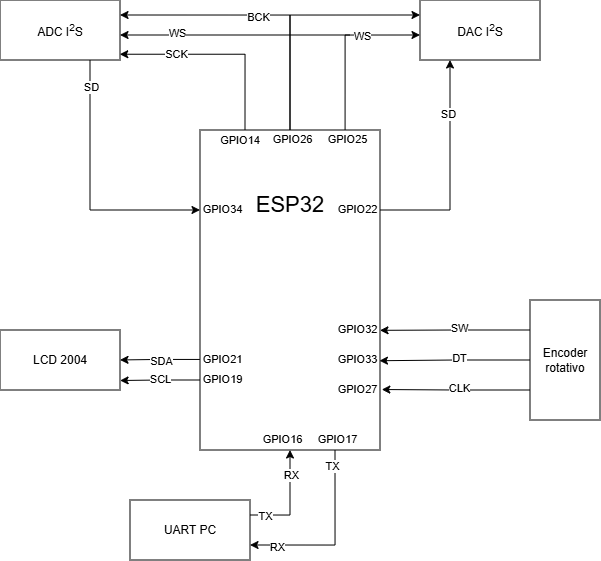
\includegraphics[width=0.65\linewidth]{Diagrama en bloques.png}
    \caption{Diagrama en bloques del sistema integrado.}
    \label{fig:diagrama_bloques}
\end{figure}

% ============================================================
\section{Hardware}
\subsection{ADC I2S PCM1808}
El bloque funcional del ADC I2S estará construido en el PCB y está basado en el circuito integrado PCM1808 \cite{pcm1808}, es un ADC con protocolo de comunicación I2S con capacidad de funcionar en formato de 24 bits y frecuencias de muestreo que van de 8kHz a 96kHz y posibilidad de funcionar tanto como maestro o esclavo. En nuestro sistema funcionará como esclavo de la comunicación I2S, establecemos frecuencia de sampleo a 44.1kHz para muestrear la señal de entrada. Este se va a comunicar al microcontrolador mediante el hardware incluido I2S guardando los datos por DMA.

\begin{figure}[H]
    \centering
    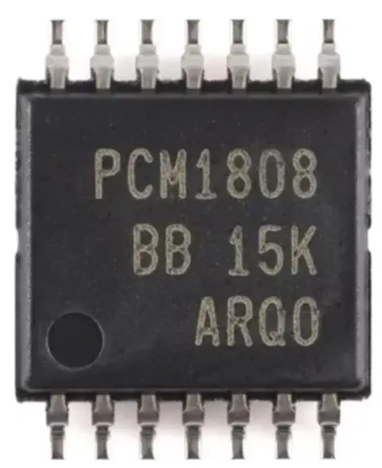
\includegraphics[width=0.25\linewidth]{PCM1808.png}
    \caption{Integrado PCM1808}
    \label{fig:pcm1808}
\end{figure}

\begin{figure}[H]
    \centering
    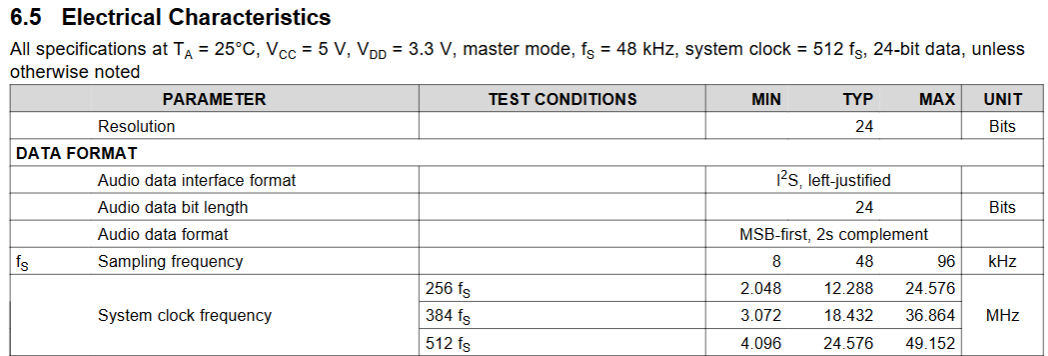
\includegraphics[width=1\linewidth]{tabla pcm1808.png}
    \caption{Tabla de parametros PCM1808}
    \label{fig:pcm1808}
\end{figure}


\subsection{DAC I2S PCM5102}
Para el DAC I2S se usará un módulo basado en el integrado PCM5102 \cite{pcm5102}, este integrado soporta resolución de palabra de 16, 24 y 32 bit, a fin de mantener la consistencia entre ADC y DAC usaremos el formato de 24 bit. También puede soportar frecuencias de  muestreo que van de 8kHz a 384kHz, la cual nuevamente se configurará a 44.1kHz por consistencia entre dispositivos. Este al igual que el ADC funcionará como esclavo de la comunicación I2S y usará los datos procesados por DSP en el microcontrolador para generar a su salida una señal analógica. Según los parámetros que da su hoja de datos tiene como máximo una salida de 2.1 Vrms con una potencia máxima de salida de 6dBm (en condición de carga mínima de 1kΩ).

\begin{figure}[H]
    \centering
    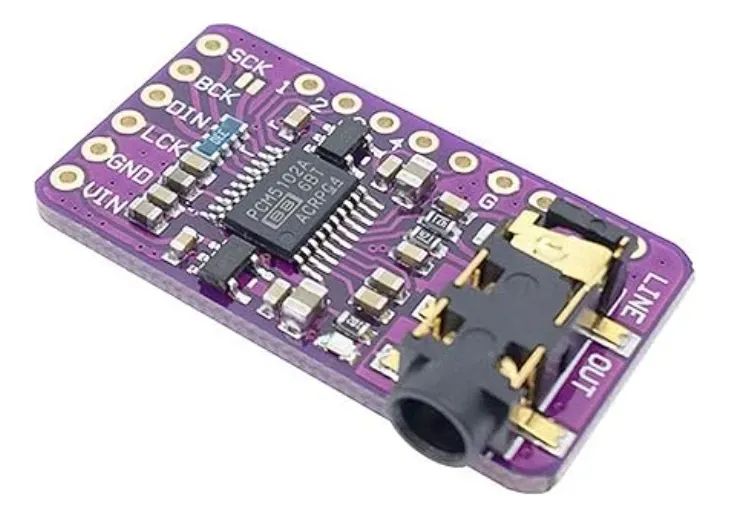
\includegraphics[width=0.3\linewidth]{PCM5102.png}
    \caption{Módulo basado en PCM5102}
    \label{fig:pcm5102}
\end{figure}

\begin{figure}[H]
    \centering
    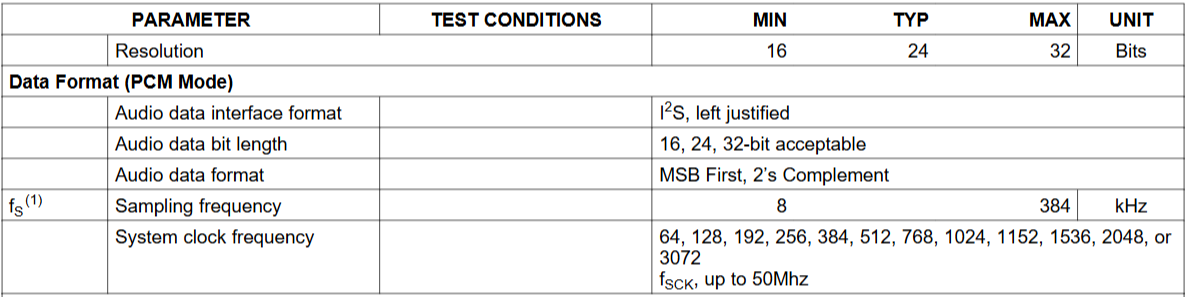
\includegraphics[width=1\linewidth]{tabla pcm5102.png}
    \caption{Tabla de parámetros PCM5102}
    \label{fig:pcm5102}
\end{figure}

\subsection{LCD 20x04}
Como elemento visual de la HMI en el prototipo se usará un display LCD de 4 filas y 20 caracteres el cual indicará la configuración actual y también contará con un cursor que indica el parámetro que se quiere modificar actualmente. Este display cuenta con un módulo adaptador de comunicación por i2C basado en el integrado PCF8574T \cite{pcf8574}.

\begin{figure}[H]
    \centering
    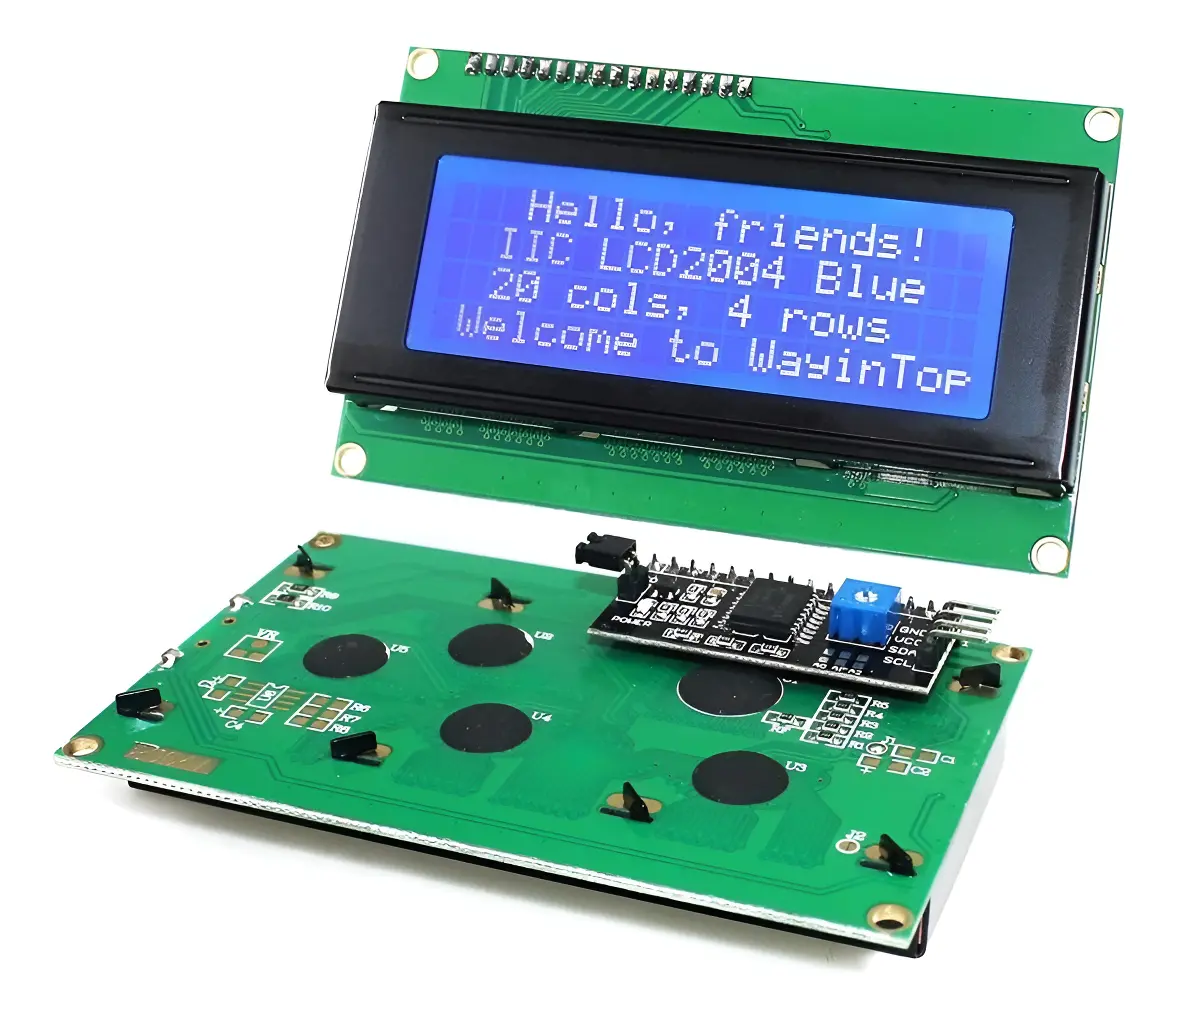
\includegraphics[width=0.4\linewidth]{LCD20x04.png}
    \caption{Frente y dorso del display LCD}
    \label{fig:lcd}
\end{figure}

\subsection{Encoder rotativo KY-040}
Como elemento interactivo se usa un encoder rotativo KY-040 \cite{ky040}.], este al ser presionado cambia la posición del cursor que indica qué parámetro se quiere modificar mientras que girarlo hará que la ganancia de la banda seleccionada por el cursor suba o baje dependiendo de si se giró en sentido horario o antihorario respectivamente.

\begin{figure}[H]
    \centering
    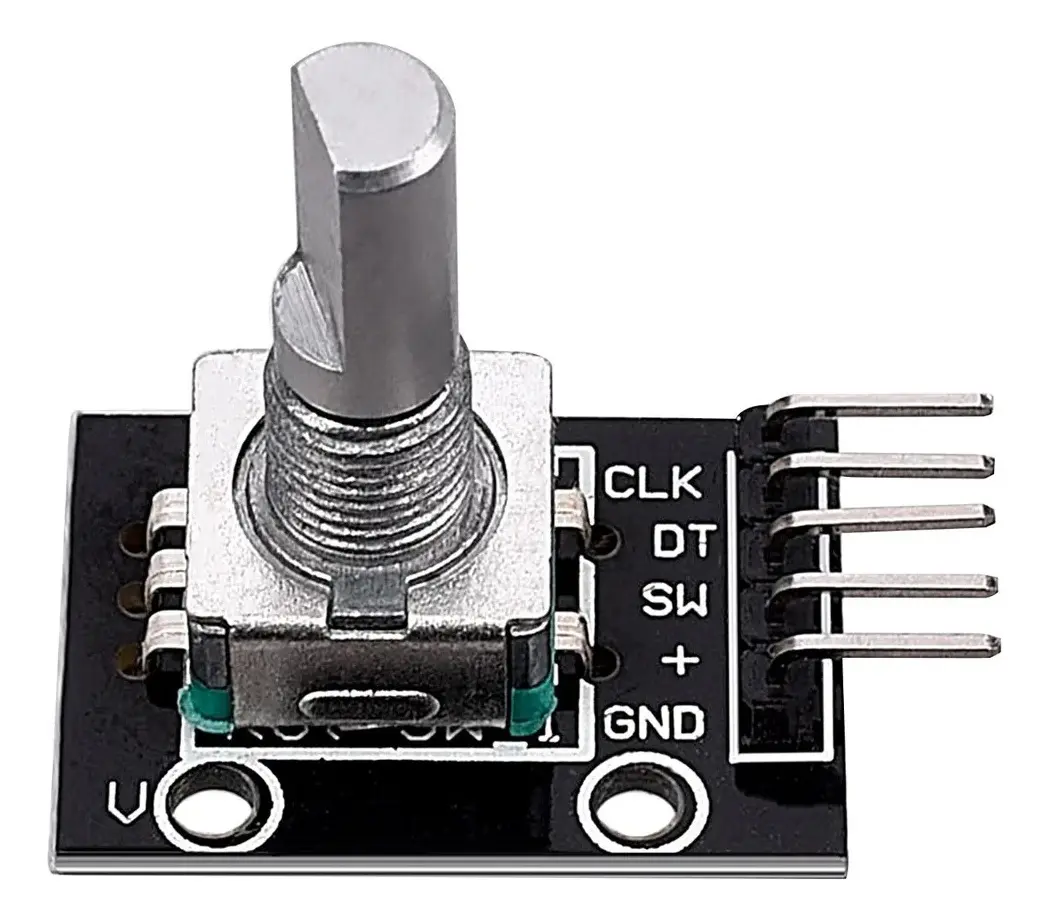
\includegraphics[width=0.3\linewidth]{encoder.png}
    \caption{Encoder rotativo KY-040}
    \label{fig:encoder}
\end{figure}

\subsection{UART PC / PL2303}
Para configuración remota se comunica una PC (o Raspberry Pi) por UART al microcontrolador. Inicialmente para la EGA se usa un conversor USB a UART basado en PL2303 \cite{pl2303}, para la EGB se usará una conexion cableada a los pines de la raspberry pi4.

\begin{figure}[H]
    \centering
    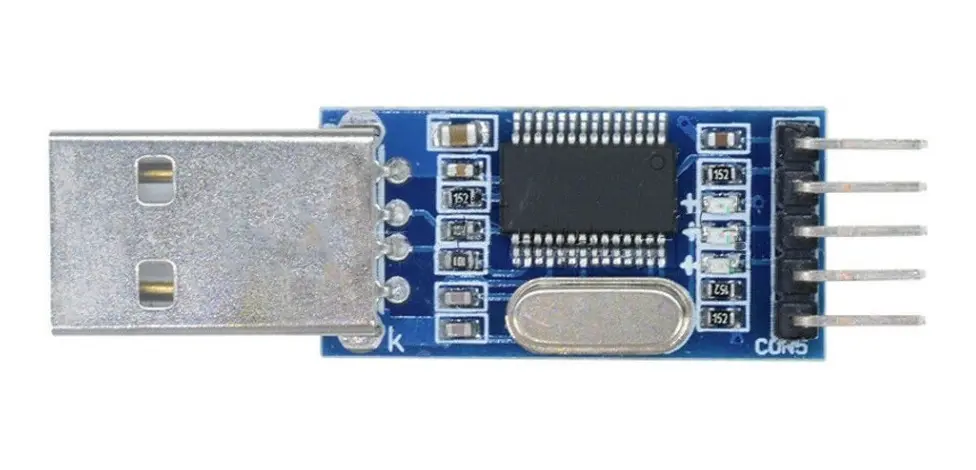
\includegraphics[width=0.4\linewidth]{PL2303.png}
    \caption{Adaptador basado en PL2303}
    \label{fig:pl2303}
\end{figure}

\subsection{ESP32}
Como centro de todo el diagrama estará el microcontrolador ESP32. Este se encargará de gestionar todos los periféricos del prototipo y del procesamiento de señales, todo por medio de un programa que hace uso de FreeRTOS
\begin{figure}[H]
    \centering
    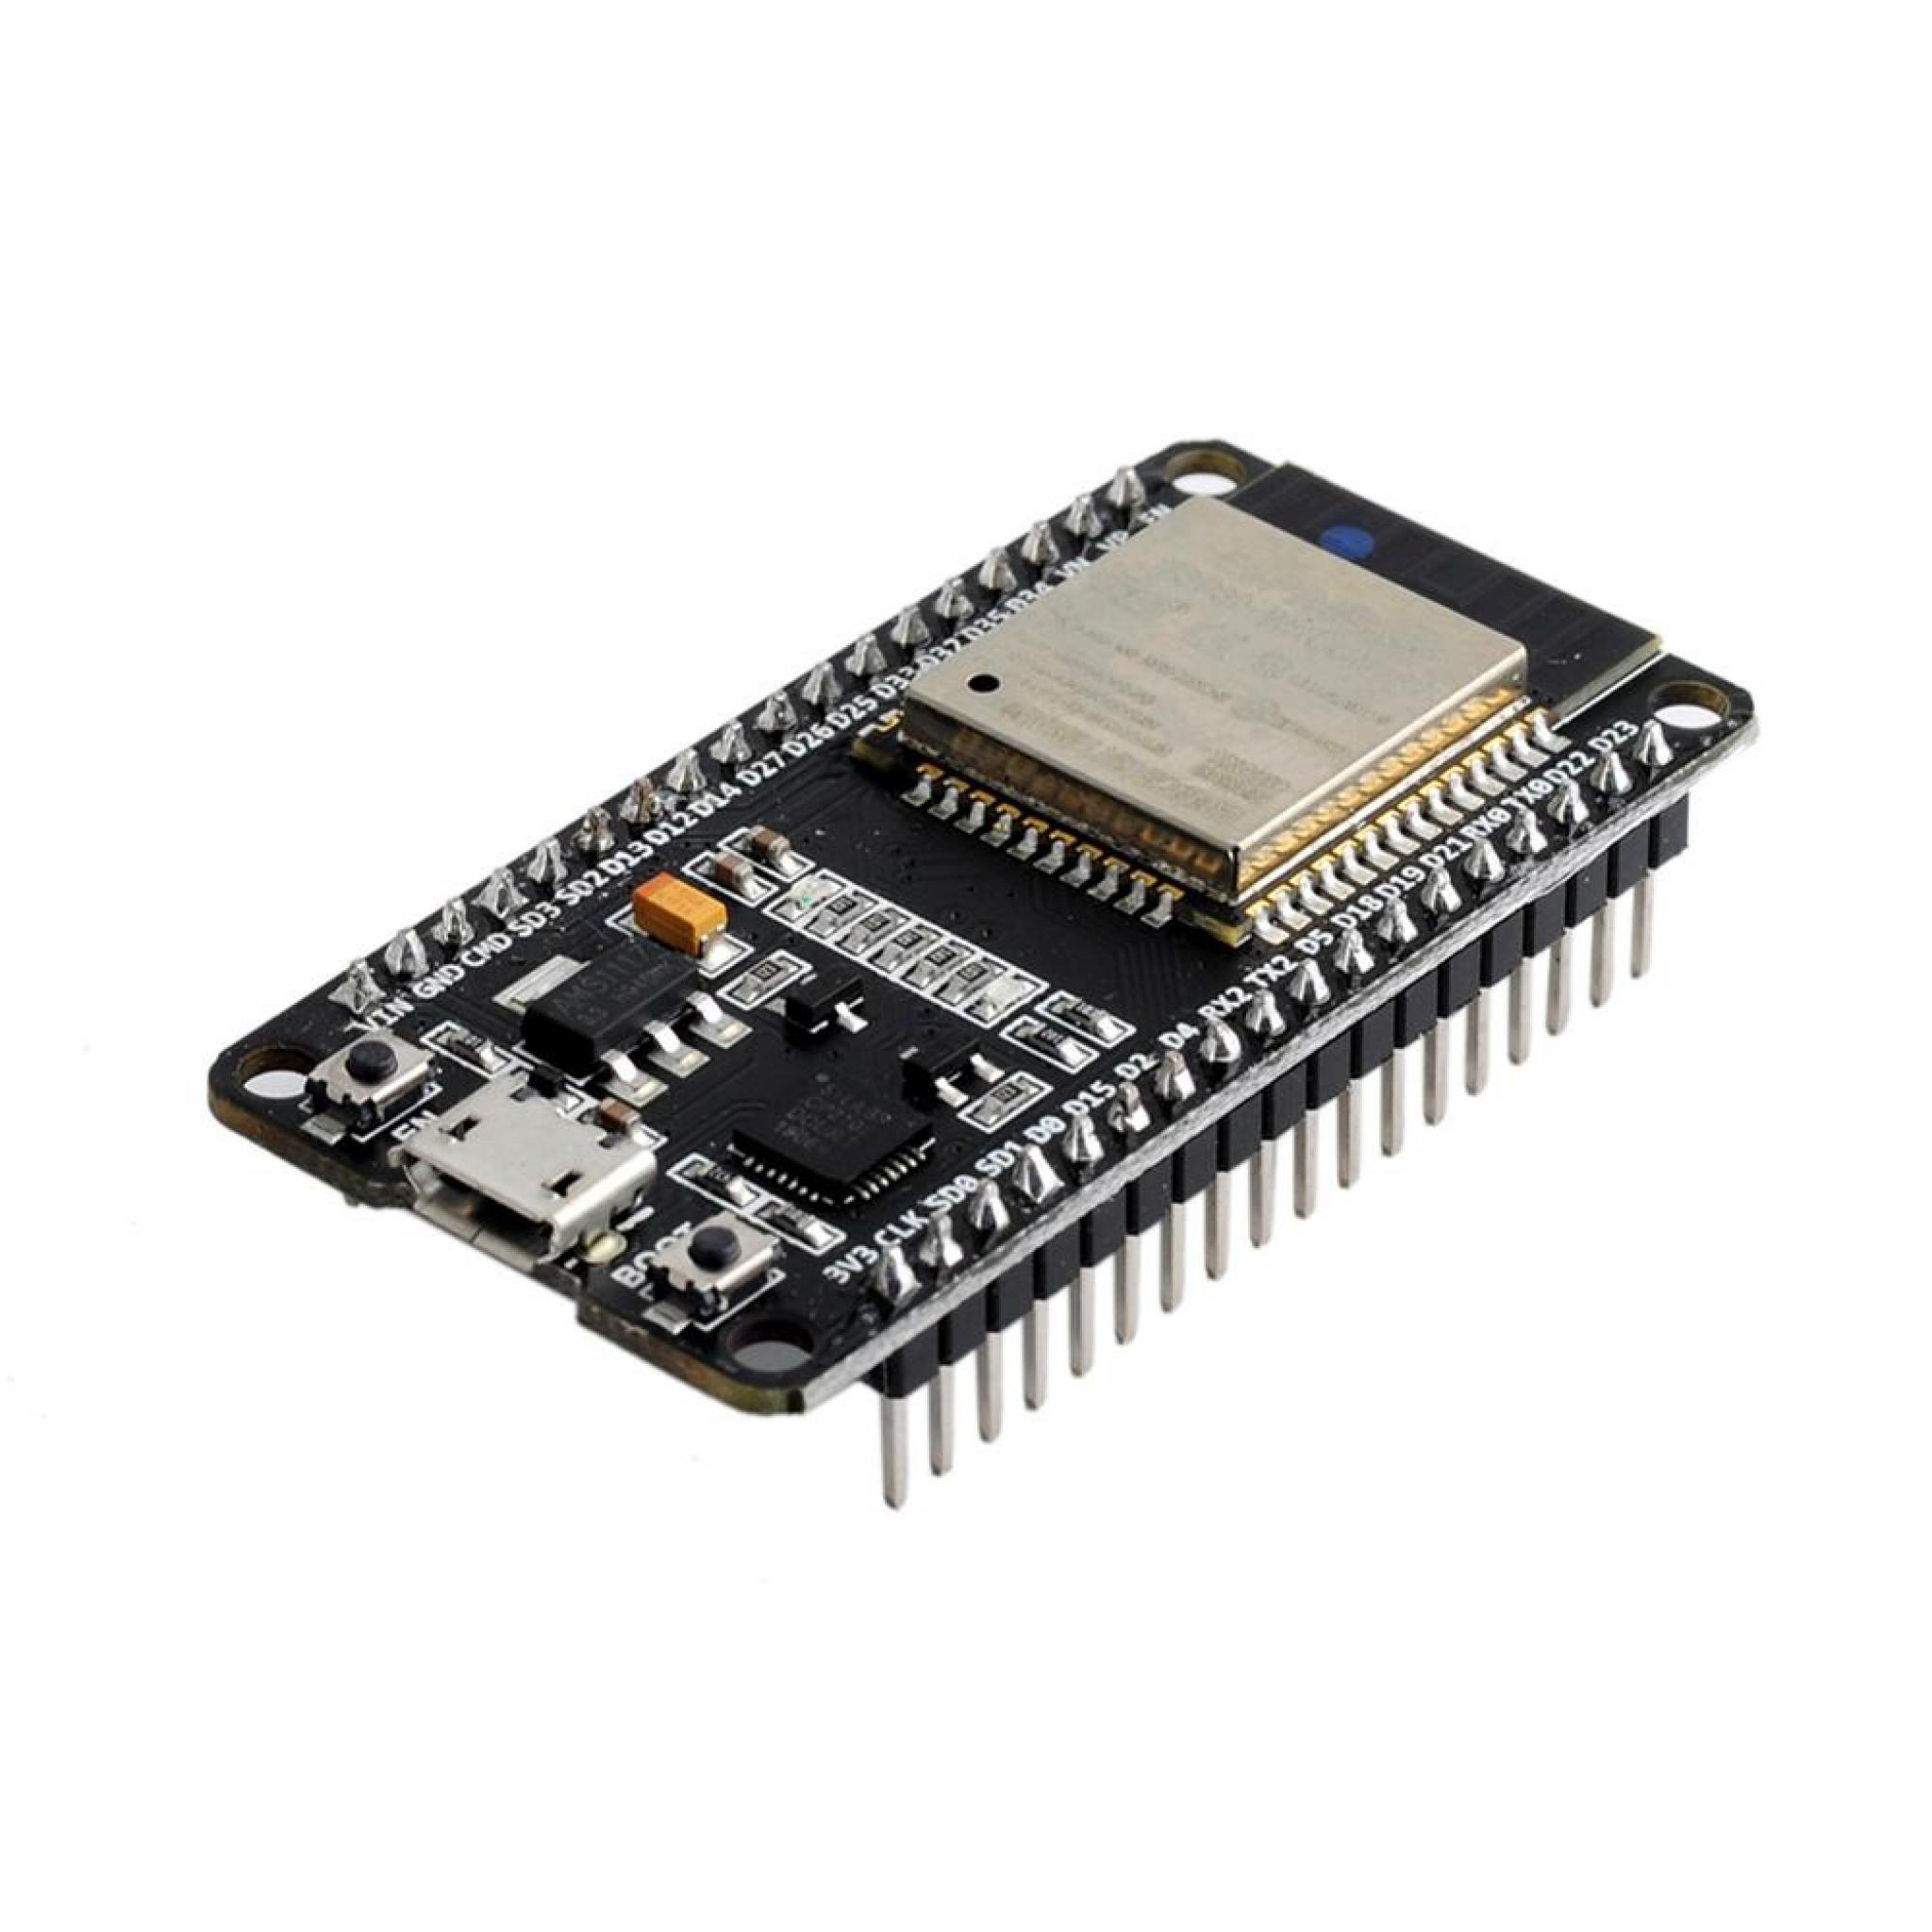
\includegraphics[width=0.4\linewidth]{ESP32.png}
    \caption{Placa de desarrollo ESP32}
    \label{fig:esp32}
\end{figure}

\subsection{Raspberry Pi 4}
Para el GPOS se utiliza una Raspberry Pi 4 como la de la figura, esta se conectará por UART al ESP32.

\begin{figure}[H]
    \centering
    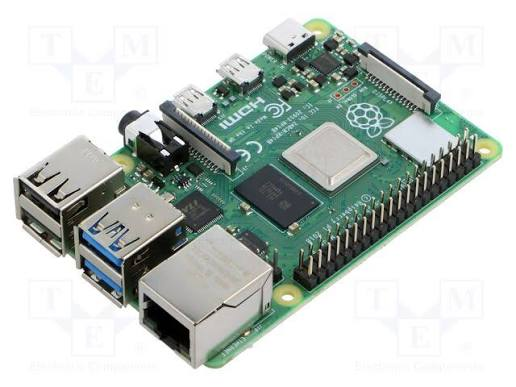
\includegraphics[width=0.6\linewidth]{raspberry.jpg}
    \caption{Raspberry Pi 4}
    \label{fig:pinout_rpi}
\end{figure}

% ============================================================
\section{Software}
\subsection{Descripción de algoritmo}
Desde el punto de vista del software el microcontrolador correrá un sistema operativo en tiempo real, más específicamente FreeRTOS provisto por ESPRESIF, el programa estará compuesto por un total de 6 tareas con 4 niveles de prioridad distribuidas entre los 2 núcleos del microcontrolador.

Primero determinaremos el funcionamiento del procesamiento y luego hablaremos propiamente de las tareas. Para hacer el procesamiento de señal el sistema consiste de un triple buffer rotativo, en simultáneo suceden 3 cosas: un buffer acumula las muestras entregadas por el ADC mediante el DMA del periférico I2S; un buffer es leído y procesado por algoritmos DSP con el núcleo del ESP32 apoyándonos en la biblioteca ESP‑DSP de Espressif, que proporciona funciones optimizadas para el núcleo Xtensa del ESP32, el contenido del buffer será reemplazado con la información procesada; y el último buffer envía los datos procesados al DAC mediante el DMA del periférico. Finalmente cada vez que el ADC llena un buffer y a su vez el DAC vacía el suyo (por tener frecuencias y tamaño de palabra coherentes), los buffer rotan, pasando el lleno del ADC a ser procesado, el procesado del DSP a salir por el DAC y el vaciado del DAC a ser llenado por el ADC.

\begin{figure}[H]
    \centering
    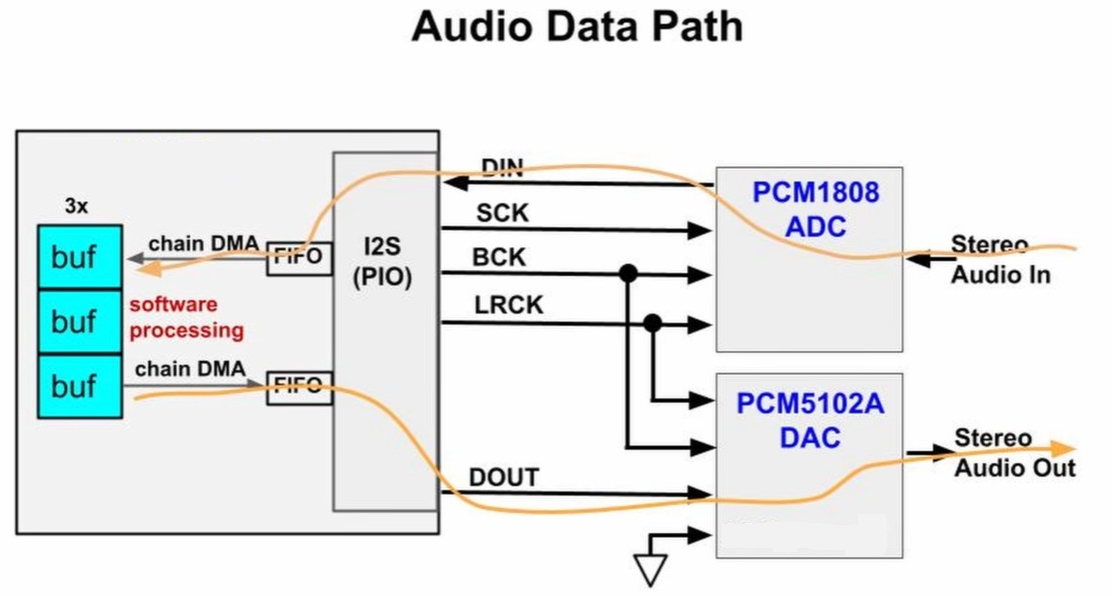
\includegraphics[width=0.6\linewidth]{datapath_audio.png}
    \caption{Datapath audio}
    \label{fig:pinout_rpi}
\end{figure}

\subsection{Tareas}
Como se dijo previamente el software del ecualizador implementa FreeRTOS con 6 tareas distribuidas en 2 núcleos según el siguiente diagrama de tareas:

\begin{figure}[H]
    \centering
    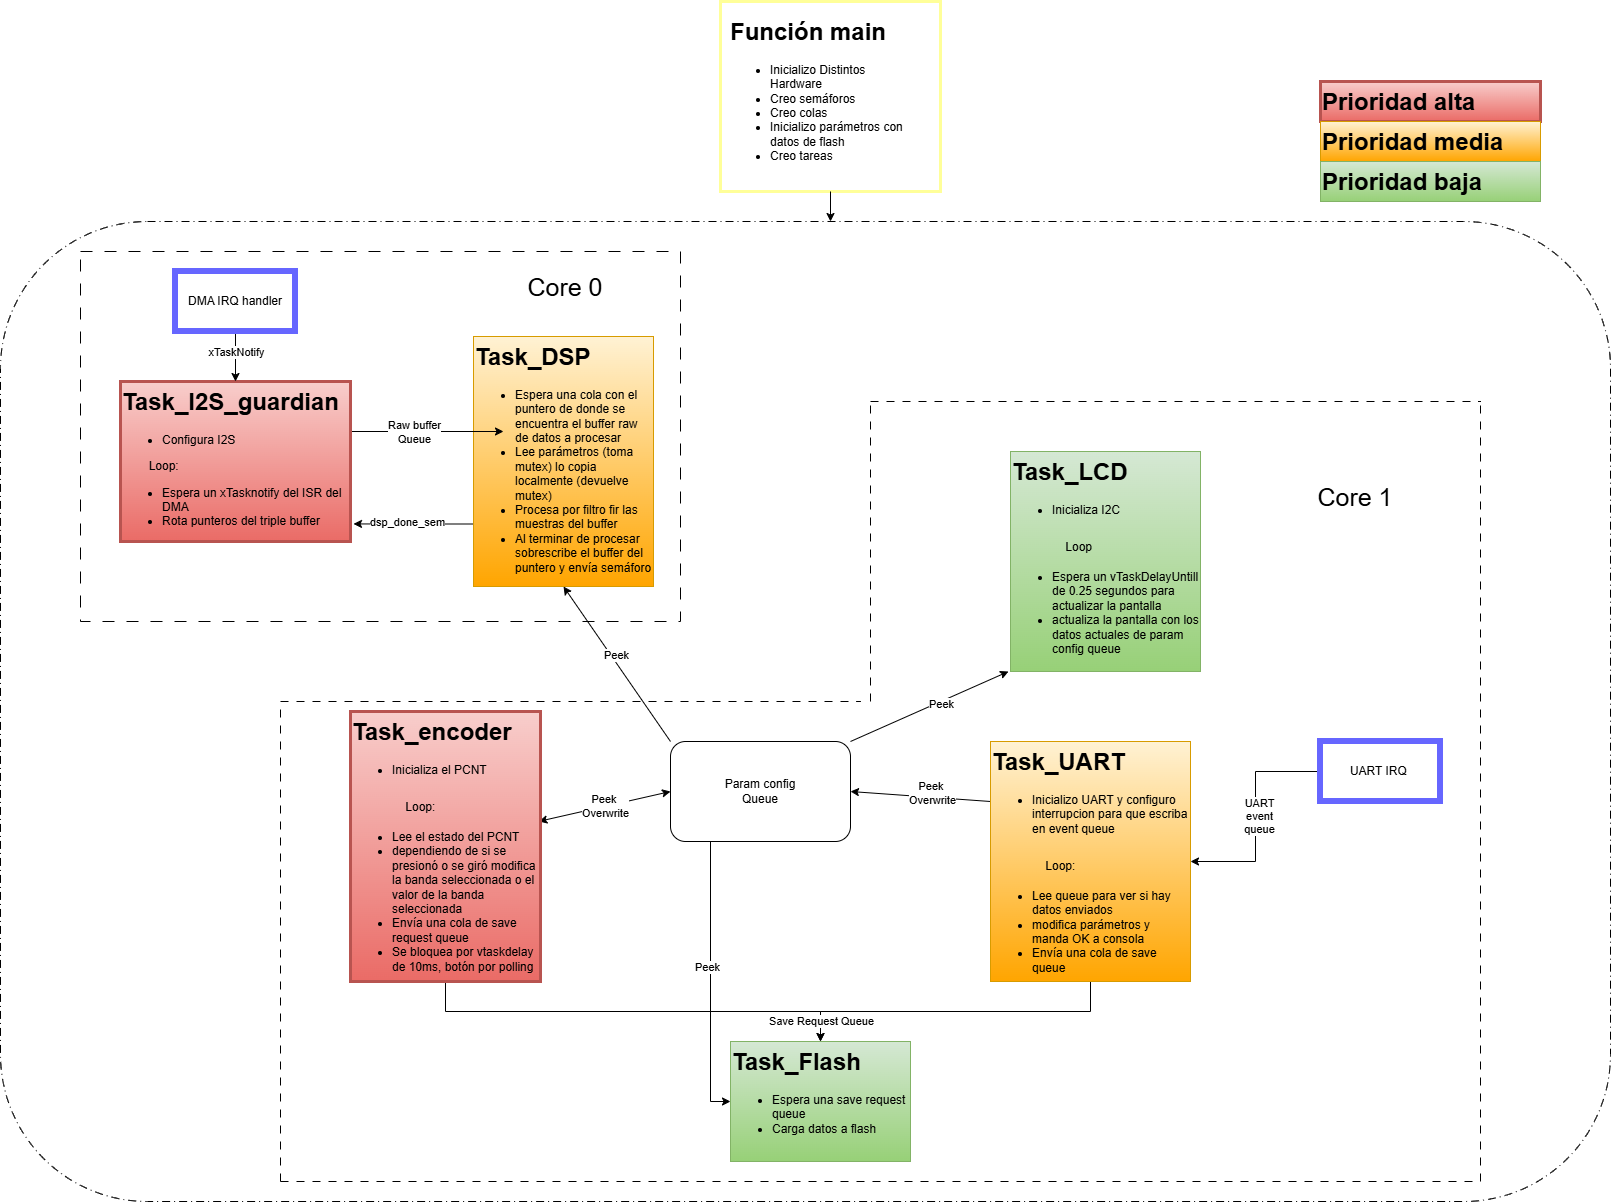
\includegraphics[width=1\linewidth]{Diagrama de tareas.png}
    \caption{Diagrama de tareas del RTOS actualizado (incluye Task\_UART para GPOS)}
    \label{fig:tareas}
\end{figure}

\subsubsection{Descripción de tareas}
\begin{itemize}
    \item \textbf{Task\_Guardian\_I2S (prioridad alta, core 0):} es la responsable exclusiva de las operaciones de lectura escritura sobre el periférico I2S y de la rotación del triple buffer. Se despierta mediante una notificación desde la ISR de recepción del DMA. Tras leer el buffer del ADC y escribir el buffer procesado al DAC, espera a que la tarea DSP termine de procesar el buffer anterior mediante el semáforo dsp\_done\_sem, y luego rota los punteros. Como sincronización para despertar usa un task notification del DMA, usado por su alta velocidad frente a un semáforo \cite{task_not}.
    \item \textbf{Task\_DSP (prioridad media, core 0):} su finalidad será procesar los datos provistos por el buffer del ADC por medio de filtros FIR propios de la librería ESP-DSP de Espressif, los cuales cuentan con operaciones optimizadas para el núcleo Xtensa del ESP32 \cite{gcc_aligned, esp_dsp_fir, esp_dsp_speed}. Cada filtro tendrá sus coeficientes calculados por medio de una función dentro del programa que usa la fórmula y método provisto en la nota de aplicación de Analog Devices para la implementación digital de un filtro Windowed-Sinc \cite{smith_windowed_sinc}. Esta tarea, a la salida de los filtros, le aplicará la ganancia correspondiente según la configuración, la cual leerá con un \texttt{xQueuePeek} de la cola de acceso común \texttt{param\_config\_queue} para finalmente ser recombinados en una sola. La sincronización de esta tarea será por un \texttt{xQueueReceive}, la cola proviene de la tarea guardiana del I2S y cuyo contenido es un puntero al buffer donde están los datos que envió el ADC, y le entregará un semáforo binario a la tarea guardiana para indicarle que finalizó de procesar los datos.
    \item \textbf{Task\_LCD (prioridad baja, core 1):} Actualiza la pantalla LCD 20 x 4 cada 250ms. Lee la configuración actual de param\_config\_queue con xQueuePeek y muestra los valores de ganancia de las tres bandas, junto con un cursor (<) que indica cuál está seleccionada. La comunicación I2C se realiza con la API estándar de ESP-IDF. Esta tarea se sincroniza con un vTaskDelayUntill() que le da ese tiempo de 250ms de refresco.
    \item \textbf{Task\_Encoder (prioridad alta, core 1):} Utiliza el módulo PCNT (Pulse Counter) provisto por espresif para el ESP32 para decodificar los pulsos de un encoder rotativo de tipo Gray. El contador se configura para incrementar o decrementar según la fase de las señales CLK y DT, eliminando la necesidad de ISRs por cada flanco. Cada vez que se acumulan una determinada cantidad de pulsos, se modifica la ganancia de la banda seleccionada (en pasos de 1dB) y se escribe el nuevo estado en param\_config\_queue mediante xQueueOverwrite. El pulsador (SW) se lee por polling con un antirrebote de 200ms y cambia la banda activa. Tiene un bloqueo cada 10ms con un vTaskDelay.
    \item \textbf{Task\_UART (prioridad media, core 1):} Instala el driver UART y procesa comandos enviados desde una terminal. Los comandos tienen el formato: set <banda> <valor> para el seteo de ganancia de una banda determinada, exec <comando> para ejecutar algunas macros como perfiles predeterminados o seteos multibanda y get <banda> que retorna valor actual en dB de la banda consultada. En base a lo recibido realizará las modificaciones indicadas en “param config queue” mediante xQueueOverwrite. La sincronización de esta tarea será por medio de un xQueueReceive de una cola llamada “UART\_event\_queue” que contendrá la información enviada desde la terminal y en base a ello actuará. Esta tarea también entregará el semáforo llamado “change\_semaphore” que indica que se hizo un cambio en la cola “param config queue”.
    \item \textbf{Task\_Flash (prioridad baja, core 1):} su finalidad será tomar los parámetros actuales de “param config queue” y escribirlos en la memoria FLASH del microcontrolador para darle permanencia a la configuración entre apagados. La sincronización de esta tarea será por medio de un xSemaphoreTake de un semáforo llamado “change\_semaphore”, este lo entregan tareas que hayan modificar los parámetros de “param config queue”.
\end{itemize}

\subsection{Arquitectura GPOS (Linux)}

El sistema GPOS corre sobre una Raspberry Pi 4 con kernel 6.12.25 o superior. Se divide en dos capas: \textbf{kernel space}, donde vive un módulo que maneja directamente la UART y expone un character device, y \textbf{user space}, donde corren las aplicaciones de control. La cadena completa de software es:

\begin{center}
\texttt{ESP32 (RTOS) $\leftrightarrow$ UART $\leftrightarrow$ serdev $\leftrightarrow$ esp32\_link $\leftrightarrow$ /dev/esp32link $\leftrightarrow$ eq\_ctl $\leftrightarrow$ SSH $\leftrightarrow$ App C\#}
\end{center}

La Figura \ref{fig:software_integrado} resume la interacción entre las capas.

\begin{figure}[H]
\centering
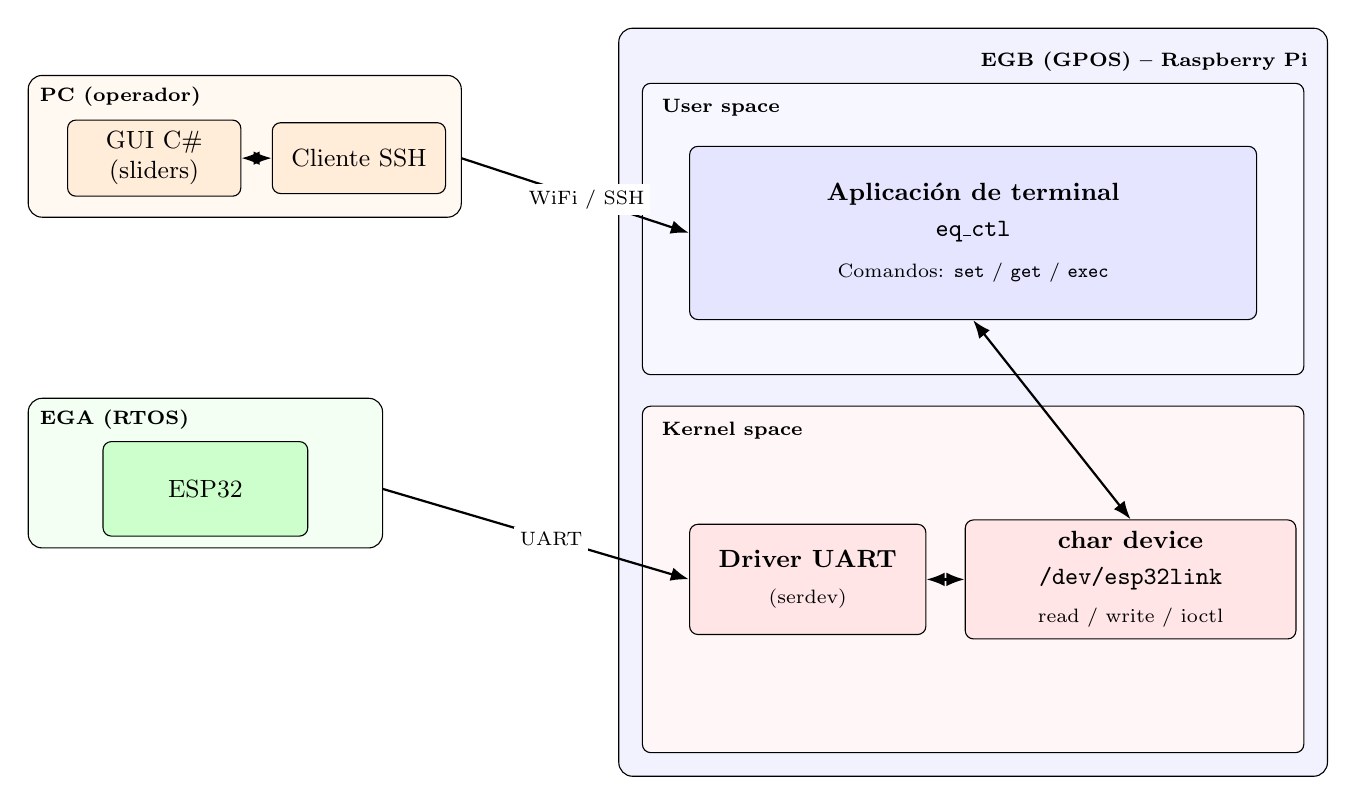
\begin{tikzpicture}[
    font=\small,
    >=Latex,
    box/.style={draw, rounded corners=3pt, align=center, inner sep=4pt,
                minimum height=9mm},
    uspace/.style={box, fill=blue!10, minimum width=20mm},
    kspace/.style={box, fill=red!10,  minimum width=20mm},
    cloud/.style={box, fill=orange!15, minimum width=22mm},
    rtos/.style={box, fill=green!20, minimum width=26mm, minimum height=12mm},
    conn/.style={->, thick},
    lbl/.style={font=\scriptsize, fill=white, inner sep=2pt}
]

% ===================== PC del operador (App C#) =====================
\draw[rounded corners=5pt, fill=orange!5] (0,5.8) rectangle (5.5,7.6);
\node[anchor=north west, font=\bfseries\scriptsize, inner sep=4pt]
    at (0,7.6) {PC (operador)};
\node[cloud] (gui) at (1.6, 6.55) {GUI C\#\\(sliders)};
\node[cloud] (ssh) at (4.2, 6.55) {Cliente SSH};
\draw[<->, thick] (gui) -- (ssh);

% ===================== EGA (RTOS) =====================
\draw[rounded corners=5pt, fill=green!5] (0,1.6) rectangle (4.5,3.5);
\node[anchor=north west, font=\bfseries\scriptsize, inner sep=4pt]
    at (0,3.5) {EGA (RTOS)};
\node[rtos] (rtos) at (2.25, 2.35) {ESP32};

% ===================== EGB (GPOS) =====================
\draw[rounded corners=5pt, fill=blue!5] (7.5,-1.3) rectangle (16.5,8.2);
\node[anchor=north east, font=\bfseries\scriptsize, inner sep=4pt]
    at (16.4, 8.05) {EGB (GPOS) -- Raspberry Pi};

% --- User space ---
\draw[rounded corners=3pt, fill=blue!3] (7.8,3.8) rectangle (16.2,7.5);
\node[anchor=north west, font=\bfseries\scriptsize, inner sep=4pt]
    at (7.9,7.45) {User space};
\node[uspace, minimum width=72mm, minimum height=22mm] (cli) at (12.0, 5.6)
    {\textbf{Aplicación de terminal}\\[2pt]
     \texttt{eq\_ctl}\\[4pt]
     \scriptsize Comandos: \texttt{set} / \texttt{get} / \texttt{exec}};

% --- Kernel space ---
\draw[rounded corners=3pt, fill=red!3] (7.8,-1.0) rectangle (16.2,3.4);
\node[anchor=north west, font=\bfseries\scriptsize, inner sep=4pt]
    at (7.9,3.35) {Kernel space};

\node[kspace, minimum width=30mm, minimum height=14mm] (drv) at ( 9.9, 1.2)
    {\textbf{Driver UART}\\[2pt]\scriptsize (serdev)};

\node[kspace, minimum width=42mm, minimum height=14mm] (chr) at (14.0, 1.2)
    {\textbf{char device}\\[2pt]
     \texttt{/dev/esp32link}\\[3pt]
     \scriptsize read / write / ioctl};

% ===================== Conexiones =====================
\draw[conn] (5.5, 6.55) -- node[lbl, pos=0.55]{WiFi / SSH} (cli.west);
\draw[conn] (4.5, 2.35) -- node[lbl, pos=0.55]{UART} (drv.west);
\draw[<->, thick] (cli.south) -- (chr.north);
\draw[<->, thick] (drv.east) -- (chr.west);

\end{tikzpicture}
\caption{Diagrama de software integrado EGA+EGB.}
\label{fig:software_integrado}
\end{figure}

\subsubsection{Kernel space: driver UART basado en serdev}

El módulo \texttt{esp32\_link.ko} se registra como driver \textit{serdev} asociado a la UART3 de la Raspberry Pi. Se eligió \texttt{serdev} en lugar de acceder directamente al periférico UART para:

\begin{itemize}
    \item Integrarse con el subsistema TTY del kernel mediante el modelo estándar de dispositivos.
    \item Evitar colisiones con el driver nativo de la UART (\texttt{8250}).
    \item Delegar el manejo de pines y baudrate al Device Tree Overlay.
\end{itemize}

\paragraph{Estructura del driver.} El módulo se declara como \texttt{serdev\_device\_driver} con una tabla \texttt{of\_device\_id} cuyo campo \texttt{compatible} es \texttt{"td3,esp32-link"}. En \texttt{probe()} se ejecutan los siguientes pasos:

\begin{enumerate}
    \item Registro de los callbacks de serdev mediante \texttt{serdev\_device\_set\_client\_ops()}.
    \item Apertura del puerto con \texttt{serdev\_device\_open()} y configuración de baudrate (leído del DT o 115200 por defecto).
    \item Reserva del \texttt{kfifo} de recepción y de la \texttt{completion} para respuestas de \texttt{get}.
    \item Reserva dinámica de major/minor, registro del \texttt{cdev} y creación de la clase y del dispositivo (\texttt{/dev/esp32link}).
\end{enumerate}

El estado global del driver incluye:
\begin{itemize}
    \item Un \texttt{kfifo} (\texttt{rx\_fifo}) y una \texttt{waitqueue} (\texttt{rx\_wait}) para el flujo asíncrono de \texttt{read()}.
    \item Una \texttt{completion} (\texttt{get\_done}) y un \texttt{mutex} (\texttt{get\_lock}) para el flujo síncrono de \texttt{ioctl(ESP32\_GET)}.
\end{itemize}

\paragraph{Interfaz ioctl.} La interfaz con user space se define en \texttt{esp32\_link.h}. Se eligió el magic number \texttt{'y'} para evitar conflictos con otros drivers del entorno de la cátedra:

\begin{lstlisting}[language=C, caption={Interfaz ioctl (extracto de esp32\_link.h)}]
#define ESP32_VAR_NAME_MAX 16

struct esp32_var {
    char nombre[ESP32_VAR_NAME_MAX];
    int  valor;
};

#define ESP32_MAGIC 'y'
#define ESP32_SET _IOW (ESP32_MAGIC, 1, struct esp32_var)
#define ESP32_GET _IOWR(ESP32_MAGIC, 2, struct esp32_var)
\end{lstlisting}

\paragraph{Recepción de datos.} La función \texttt{esp32\_receive\_buf()} es llamada por el kernel cada vez que llegan bytes por la UART. Acumula los bytes en un \texttt{linebuf} hasta encontrar el carácter \texttt{\textbackslash n}. Cuando completa una línea:

\begin{enumerate}
    \item La publica en el \texttt{kfifo} y despierta a cualquier \texttt{read()} que esté esperando.
    \item Si hay un \texttt{ESP32\_GET} pendiente (flag \texttt{esperando\_get}), copia la línea a \texttt{get\_response} y llama a \texttt{complete(\&get\_done)}.
\end{enumerate}

\paragraph{Envío de datos.} La función \texttt{esp32\_write()} copia los datos de usuario a un buffer local, asegura el terminador \texttt{\textbackslash n} y los envía con \texttt{serdev\_device\_write()} con un timeout de 1 segundo.

\paragraph{Device Tree Overlay.} El nodo \texttt{esp32-link} se declara en \texttt{esp32-link-pi4-overlay.dts} y se cuelga de \texttt{uart3}. Los pines GPIO4 y GPIO5 se configuran en ALT4 (TXD3/RXD3) mediante un grupo de pinctrl dedicado, evitando depender del overlay oficial \texttt{uart3}:

\begin{lstlisting}[language=C, caption={Extracto del Device Tree Overlay}]
fragment@0 {
    target = <&gpio>;
    __overlay__ {
        esp32_link_pins: esp32_link_pins {
            brcm,pins = <4 5>;
            brcm,function = <3>; /* ALT4: GPIO4=TXD3, GPIO5=RXD3 */
            brcm,pull = <0 2>;   /* TX sin pull, RX con pull-up */
        };
    };
};

fragment@1 {
    target = <&uart3>;
    __overlay__ {
        pinctrl-names = "default";
        pinctrl-0 = <&esp32_link_pins>;
        status = "okay";

        esp32_link: esp32-link {
            compatible = "td3,esp32-link";
            current-speed = <115200>;
            status = "okay";
        };
    };
};
\end{lstlisting}

\paragraph{Compilación.} El Makefile del módulo genera dos artefactos: el módulo del kernel \texttt{esp32\_link.ko} y el ejecutable de usuario \texttt{eq\_ctl}:

\begin{lstlisting}[language=make, caption={Makefile del módulo y del cliente de usuario}]
KDIR := /lib/modules/$(shell uname -r)/build
MDIR := $(PWD)/build

obj-m += esp32_link.o

all: module ctl

module:
    @mkdir -p build; \
    cp -f esp32_link.c esp32_link.h Makefile $(MDIR); \
    cd build; make -C $(KDIR) M=$(MDIR) modules

ctl:
    gcc -Wall -pthread -o eq_ctl eq_ctl.c

clean:
    @cd build; make -C $(KDIR) M=$(MDIR) clean; cd ..; \
    rm -rf build eq_ctl
\end{lstlisting}

\subsubsection{User space: aplicación de terminal y aplicación gráfica}

Se desarrollaron dos aplicaciones de usuario que interactúan con \texttt{/dev/esp32link}:

\paragraph{Aplicación de terminal (\texttt{eq\_ctl}).} Programa en C que corre en la Raspberry Pi, abre el dispositivo y ofrece un prompt interactivo con tres comandos:

\begin{itemize}
    \item \texttt{set BANDA NIVEL}: usa \texttt{ioctl(ESP32\_SET)}. El driver lo traduce a \texttt{set BANDA NIVEL\textbackslash n} por la UART.
    \item \texttt{get BANDA}: usa \texttt{ioctl(ESP32\_GET)}. Bloquea hasta que el ESP32 responde con \texttt{BANDA=valor}.
    \item \texttt{exec PRESET}: usa \texttt{write()}. Se manda el texto crudo y el firmware lo interpreta como una macro multibanda.
\end{itemize}

Un hilo secundario (\texttt{hilo\_monitor}) bloquea en \texttt{read()} e imprime por consola todo lo que el ESP32 envía de forma espontánea. Un mutex (\texttt{consola}) serializa las impresiones del hilo principal y del hilo receptor para evitar mezclas en \texttt{stdout}.

\paragraph{Aplicación gráfica (cliente en C\# por SSH).} La segunda aplicación se desarrolló en C\# y corre en la PC del operador. Se conecta por SSH a la Raspberry Pi usando la librería \texttt{SSH.NET} y ejecuta remotamente el programa \texttt{eq\_ctl} en modo no interactivo, enviando comandos por \texttt{stdin}. La interfaz presenta:

\begin{itemize}
    \item Tres sliders de ganancia, uno por banda (low/mid/high), con rango de $\pm$12 dB y paso de 1 dB.
    \item Botones de presets (\texttt{rock}, \texttt{jazz}, \texttt{flat}) que ejecutan \texttt{exec <preset>}.
    \item Un panel de estado que refresca periódicamente los valores actuales mediante \texttt{get <banda>}.
    \item Indicadores de conexión SSH y del estado del driver.
\end{itemize}

Esta arquitectura en dos capas de usuario permite operar el sistema tanto de forma local (terminal) como remota (interfaz gráfica).

\section{Diseño de PCB}
\subsection{Esquemático}
El esquemático completo se muestra en la Figura \ref{fig:esquematico}. Incluye el ESP32, ADC, DAC, LCD, encoder, UART y alimentación.

\begin{figure}[H]
    \centering
    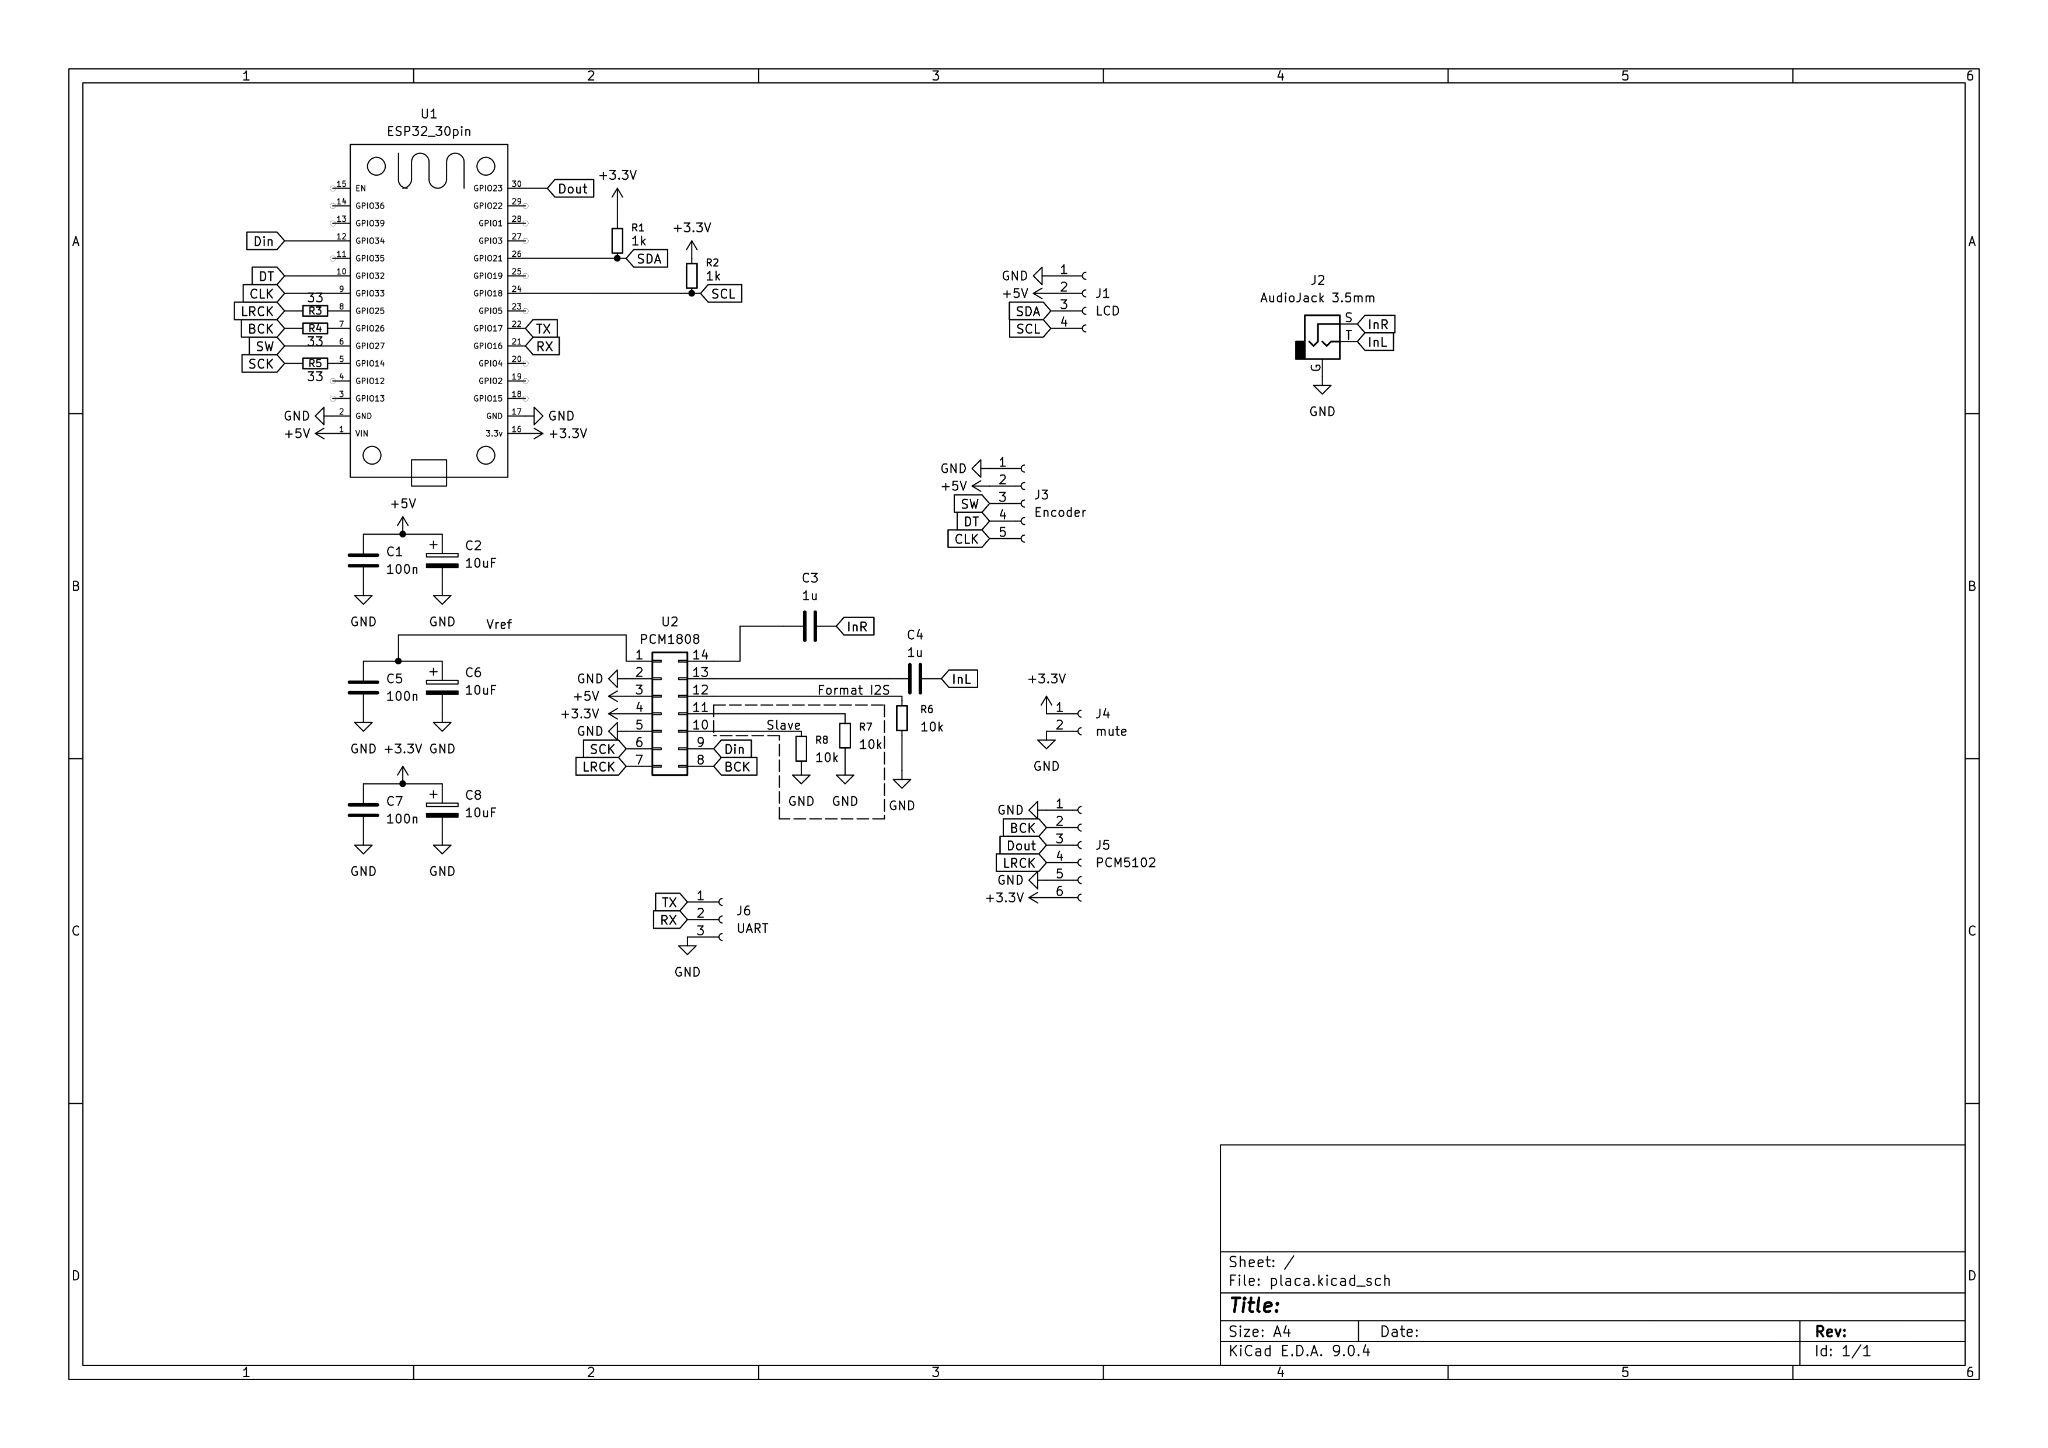
\includegraphics[width=1\linewidth]{esquemático.jpg}
    \caption{Esquemático del ecualizador}
    \label{fig:esquematico}
\end{figure}

\subsection{Layout}
El layout del PCB se muestra en la Figura \ref{fig:pcb}.

\begin{figure}[H]
    \centering
    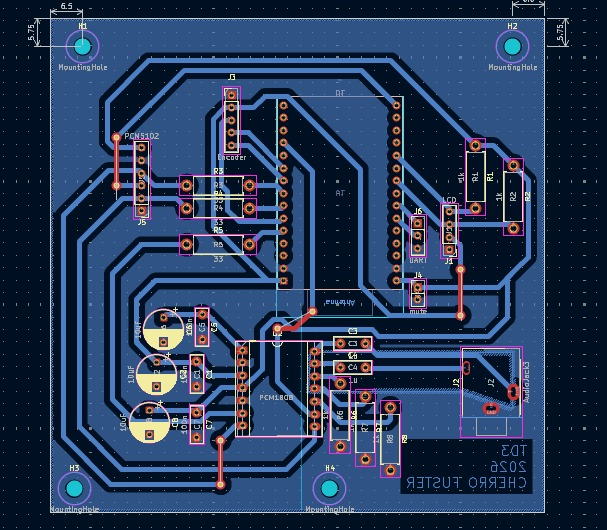
\includegraphics[width=0.7\linewidth]{PCB.png}
    \caption{Layout del PCB}
    \label{fig:pcb}
\end{figure}

\subsection{Test points}
\begin{table}[H]
\centering
\begin{tabular}{@{}lll@{}}
\toprule
Test point & Señal & Descripción \\
\midrule
TP1 & Canal izquierdo IN  & Entrada analógica del canal izquierdo \\
TP2 & Canal izquierdo OUT & Salida analógica del canal izquierdo \\
TP3 & Canal derecho IN    & Entrada analógica del canal derecho \\
TP4 & Canal derecho OUT   & Salida analógica del canal derecho \\
TP5 & GND                 & Masa de referencia \\
\bottomrule
\end{tabular}
\caption{Lista de test points del PCB.}
\label{tab:testpoints}
\end{table}

\subsection{PCB físico}
\begin{figure}[H]
    \centering
    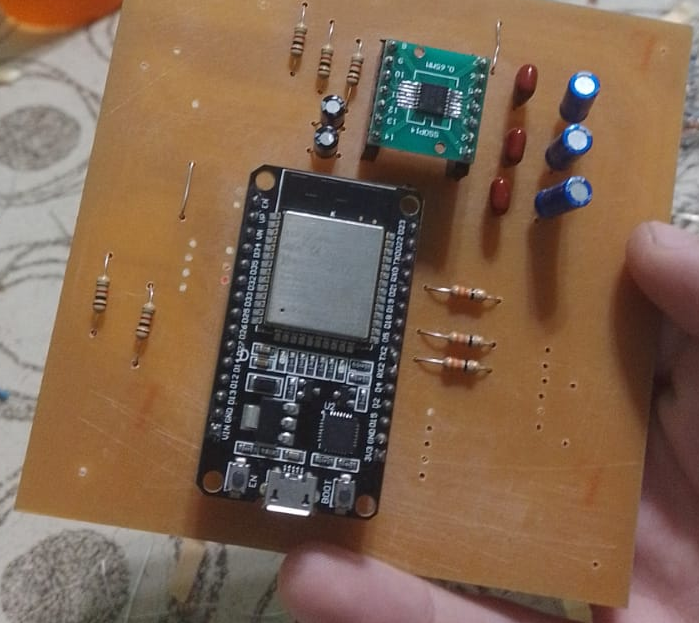
\includegraphics[width=0.5\linewidth]{pcb real.png}
    \caption{Producto final del PCB}
    \label{fig:pcb}
\end{figure}


% ============================================================
\section{Resultados y mediciones}
El ecualizador digital demostró un procesamiento en tiempo real efectivo, con una frecuencia de muestreo de 44.1 kHz y un rango de ganancia de $\pm$12 dB. Las mediciones con osciloscopio confirman la respuesta de los filtros FIR. Se configuraron ganancias en +12 dB, -12 dB y 0 dB para bajos, medios y agudos respectivamente.

\begin{figure}[H]
    \centering
    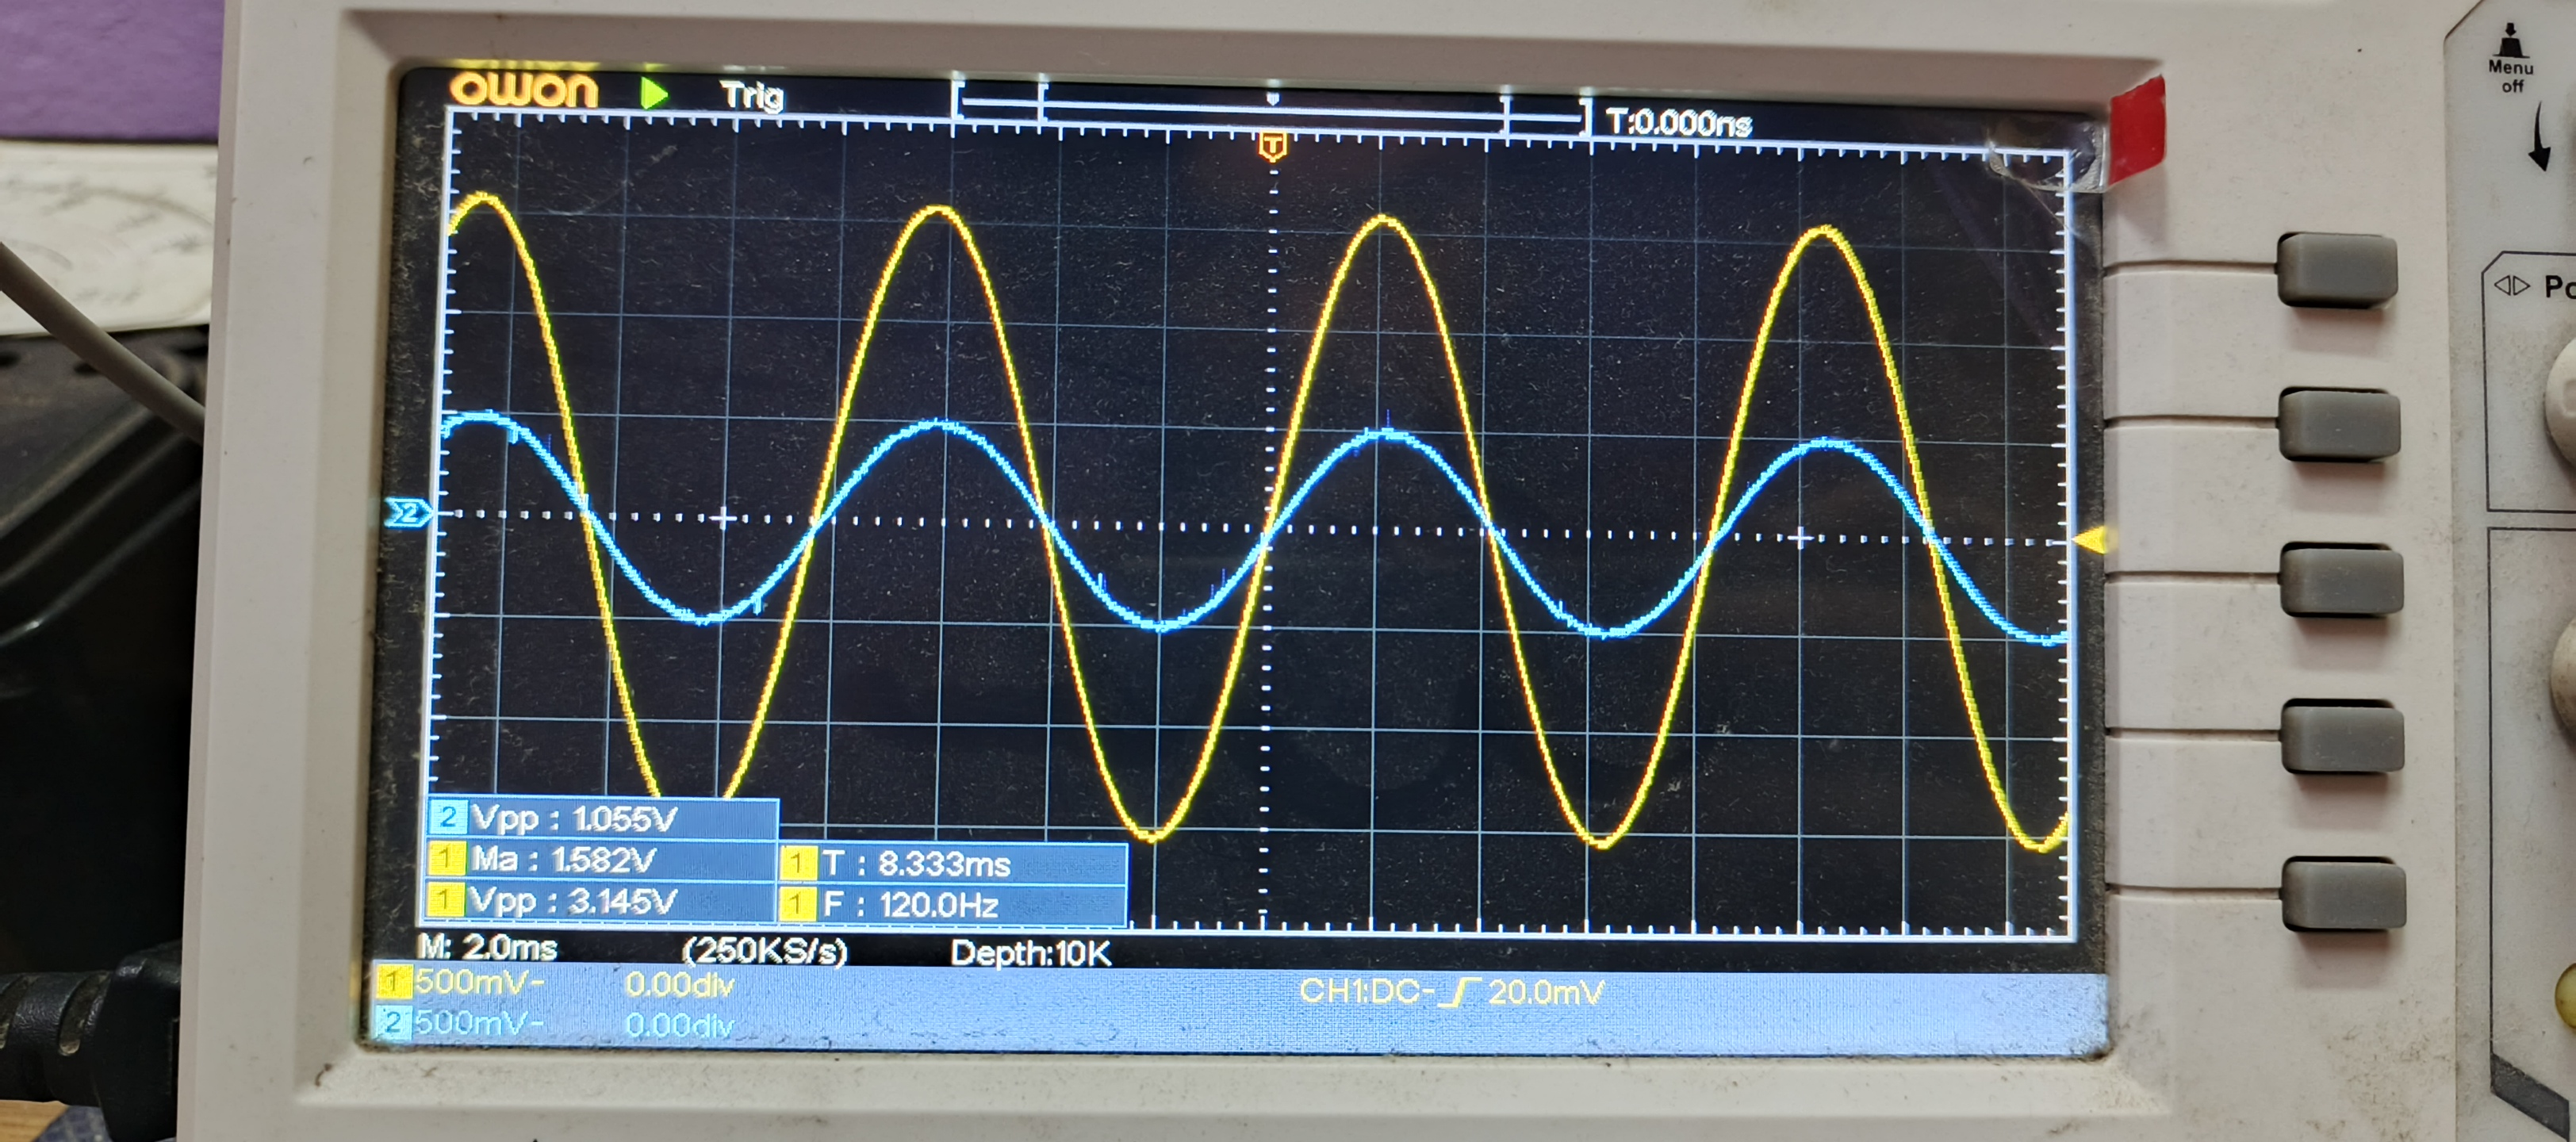
\includegraphics[width=0.6\linewidth]{120Hz+10dB.jpg}
    \caption{Captura de osciloscopio para senoidal de 120 Hz con ganancia de 10 dB}
    \label{fig:120hz}
\end{figure}

\begin{figure}[H]
    \centering
    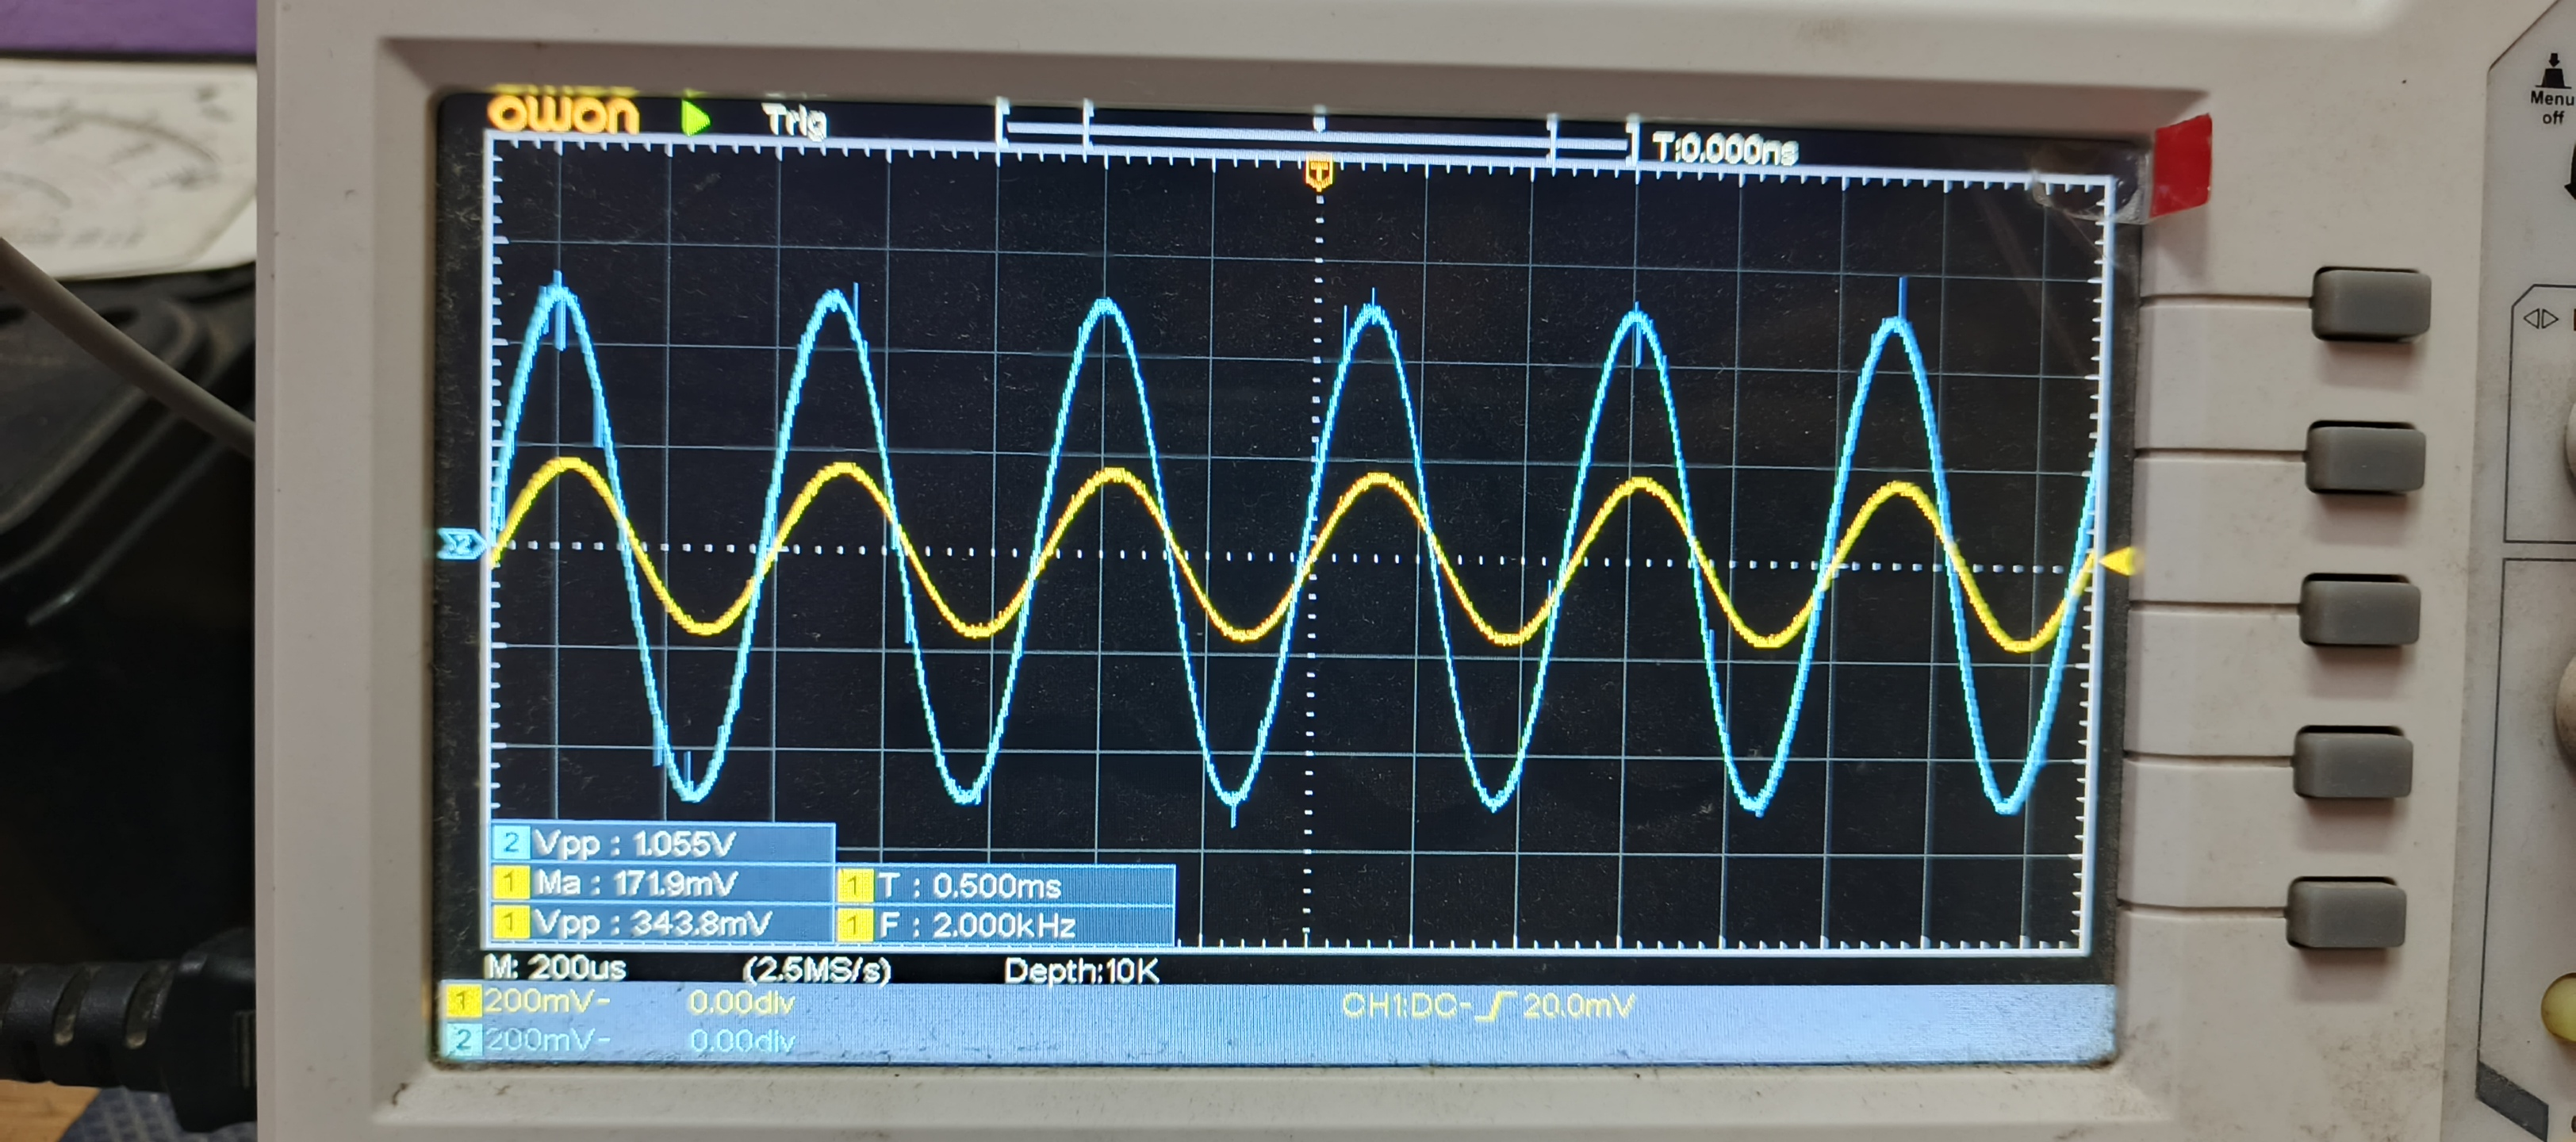
\includegraphics[width=0.6\linewidth]{2kHz-10dB.jpg}
    \caption{Captura de osciloscopio para senoidal de 2 kHz con atenuación de 10 dB}
    \label{fig:2khz}
\end{figure}

\begin{figure}[H]
    \centering
    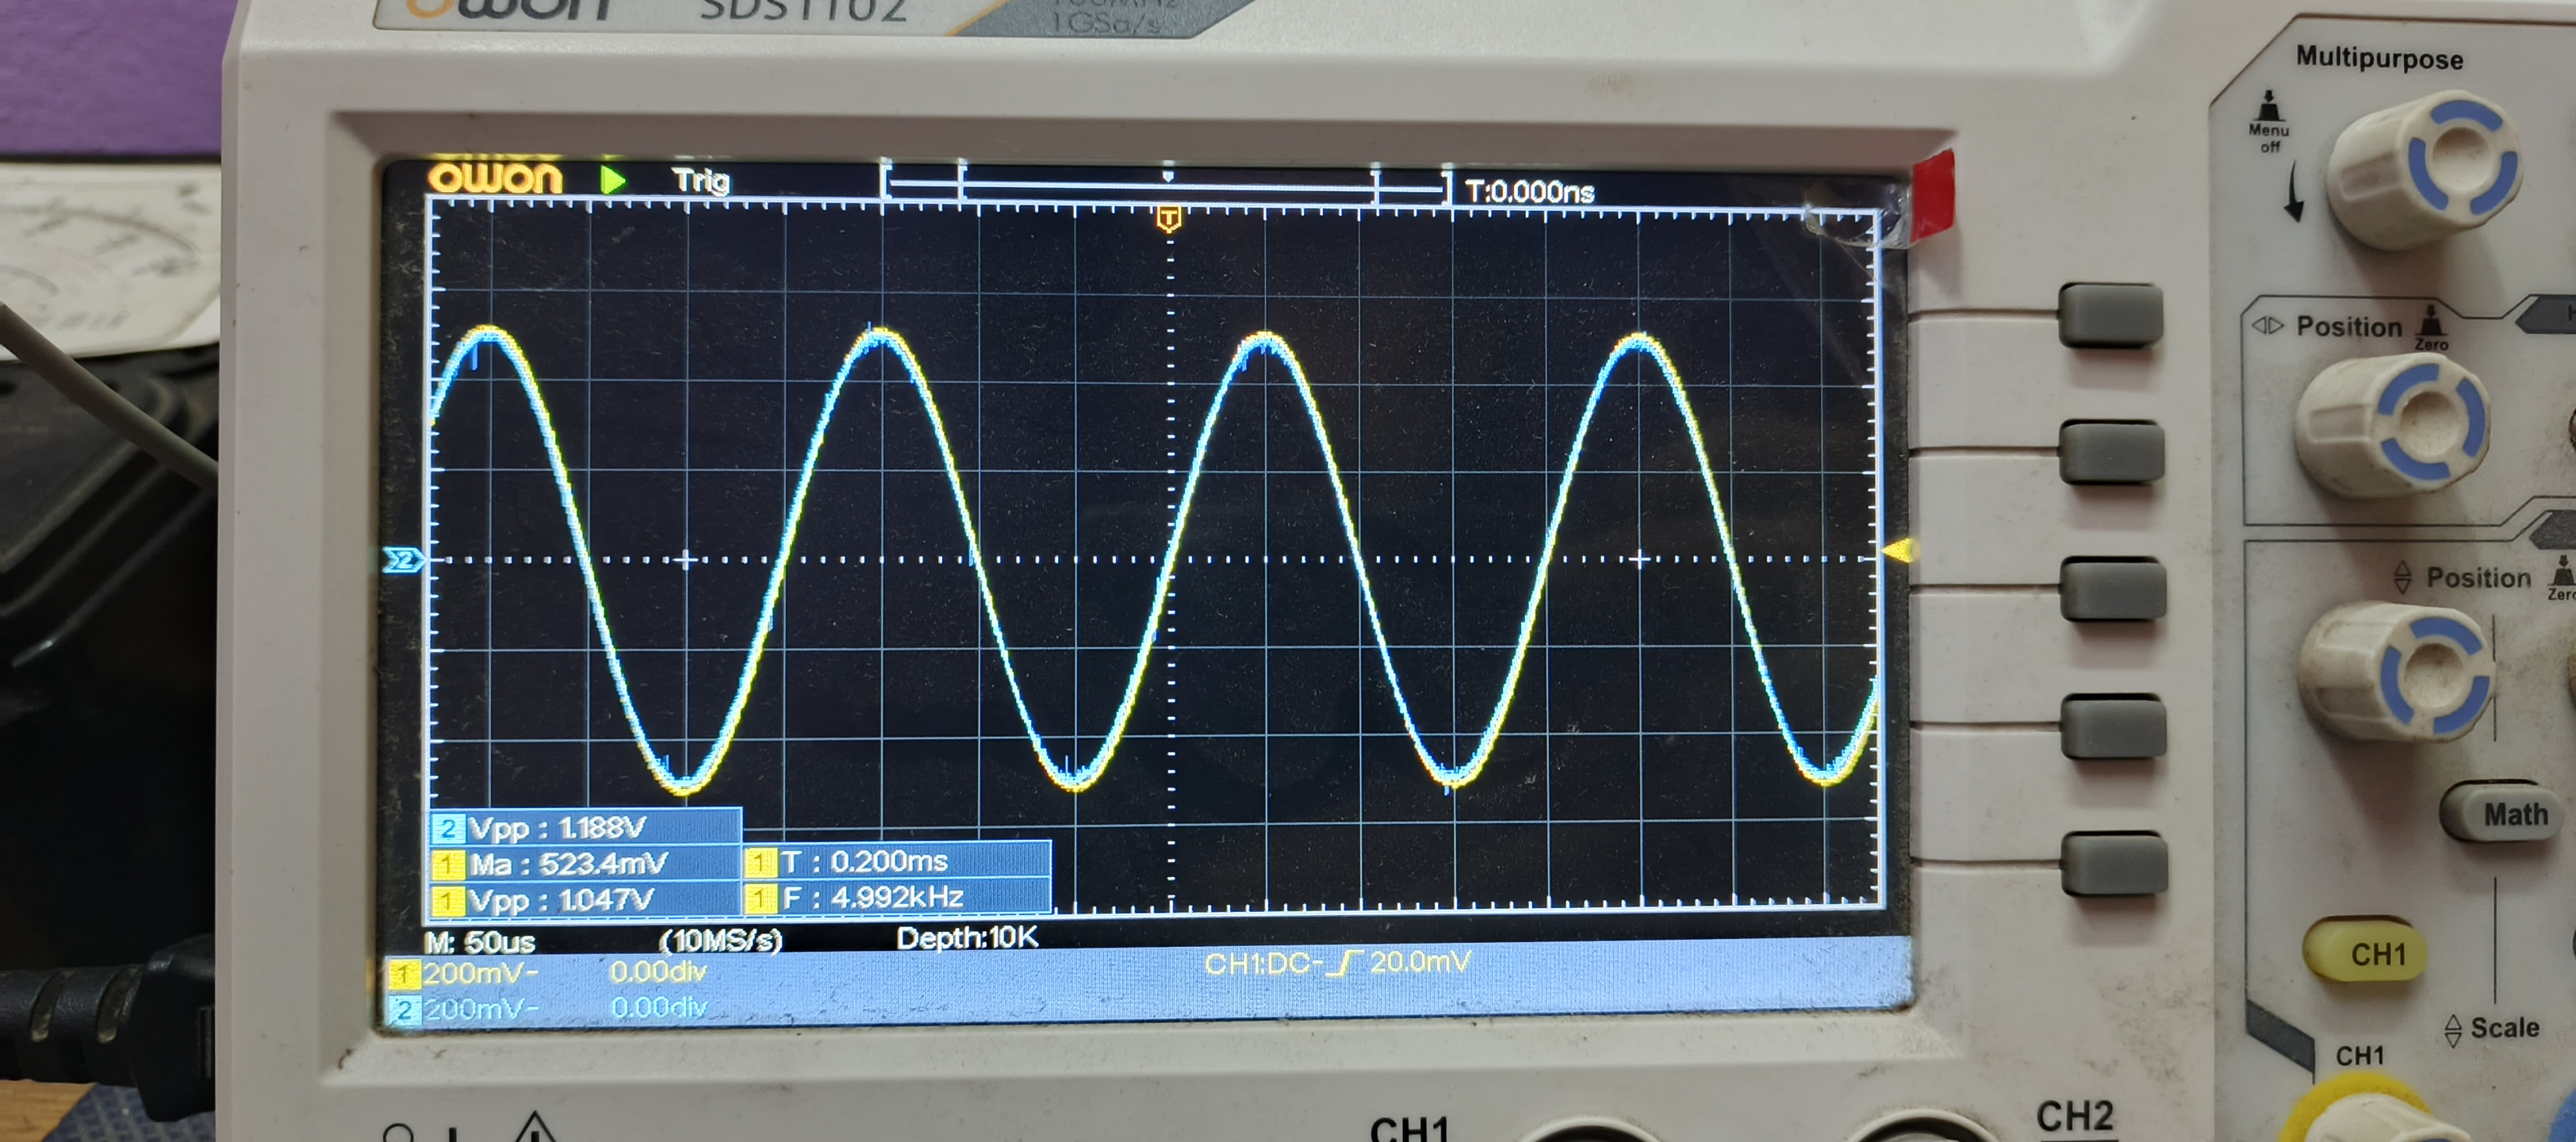
\includegraphics[width=0.6\linewidth]{5kHz0dB.jpg}
    \caption{Captura de osciloscopio para senoidal de 5 kHz sin modificar}
    \label{fig:5khz}
\end{figure}

\section{Anexo imagenes}

\begin{figure}[H]
    \centering
    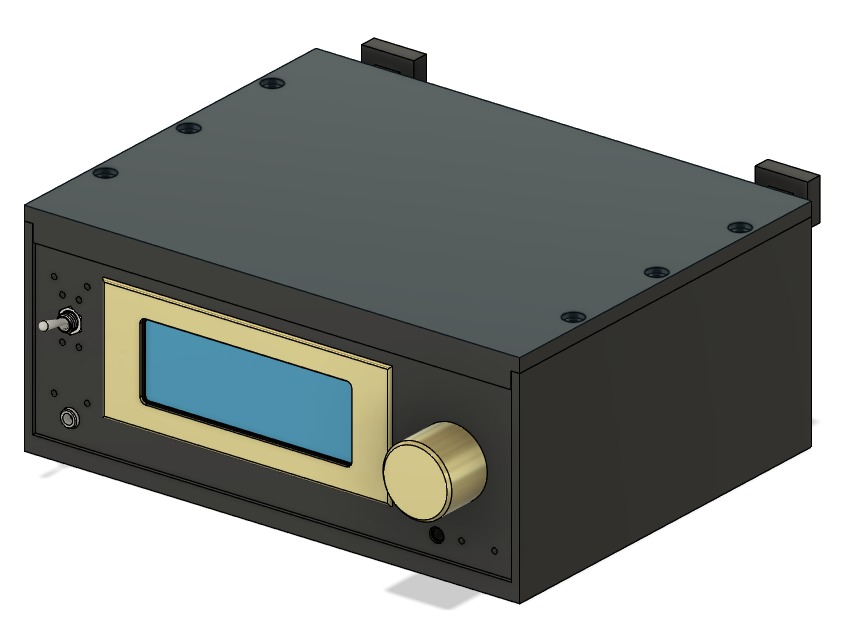
\includegraphics[width=0.7\linewidth]{Carcaza 3d.png}
    \caption{Frente modelo 3D Carcaza}
    \label{fig:}
\end{figure}

\begin{figure}[H]
    \centering
    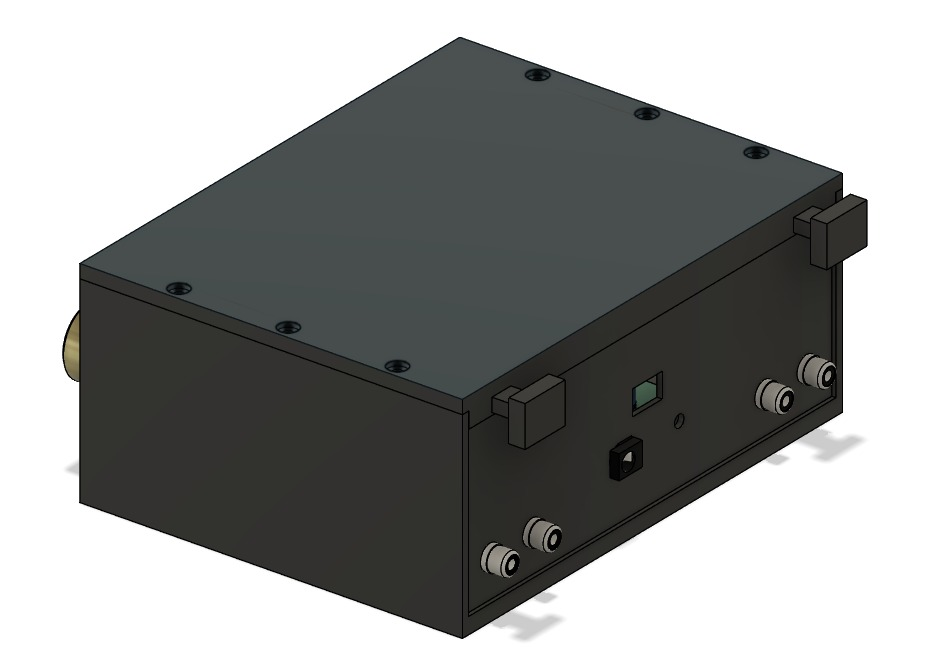
\includegraphics[width=0.7\linewidth]{Carcaza 3d atras.png}
    \caption{Reverso modelo 3D Carcaza}
    \label{fig:}
\end{figure}

\begin{figure}[H]
    \centering
    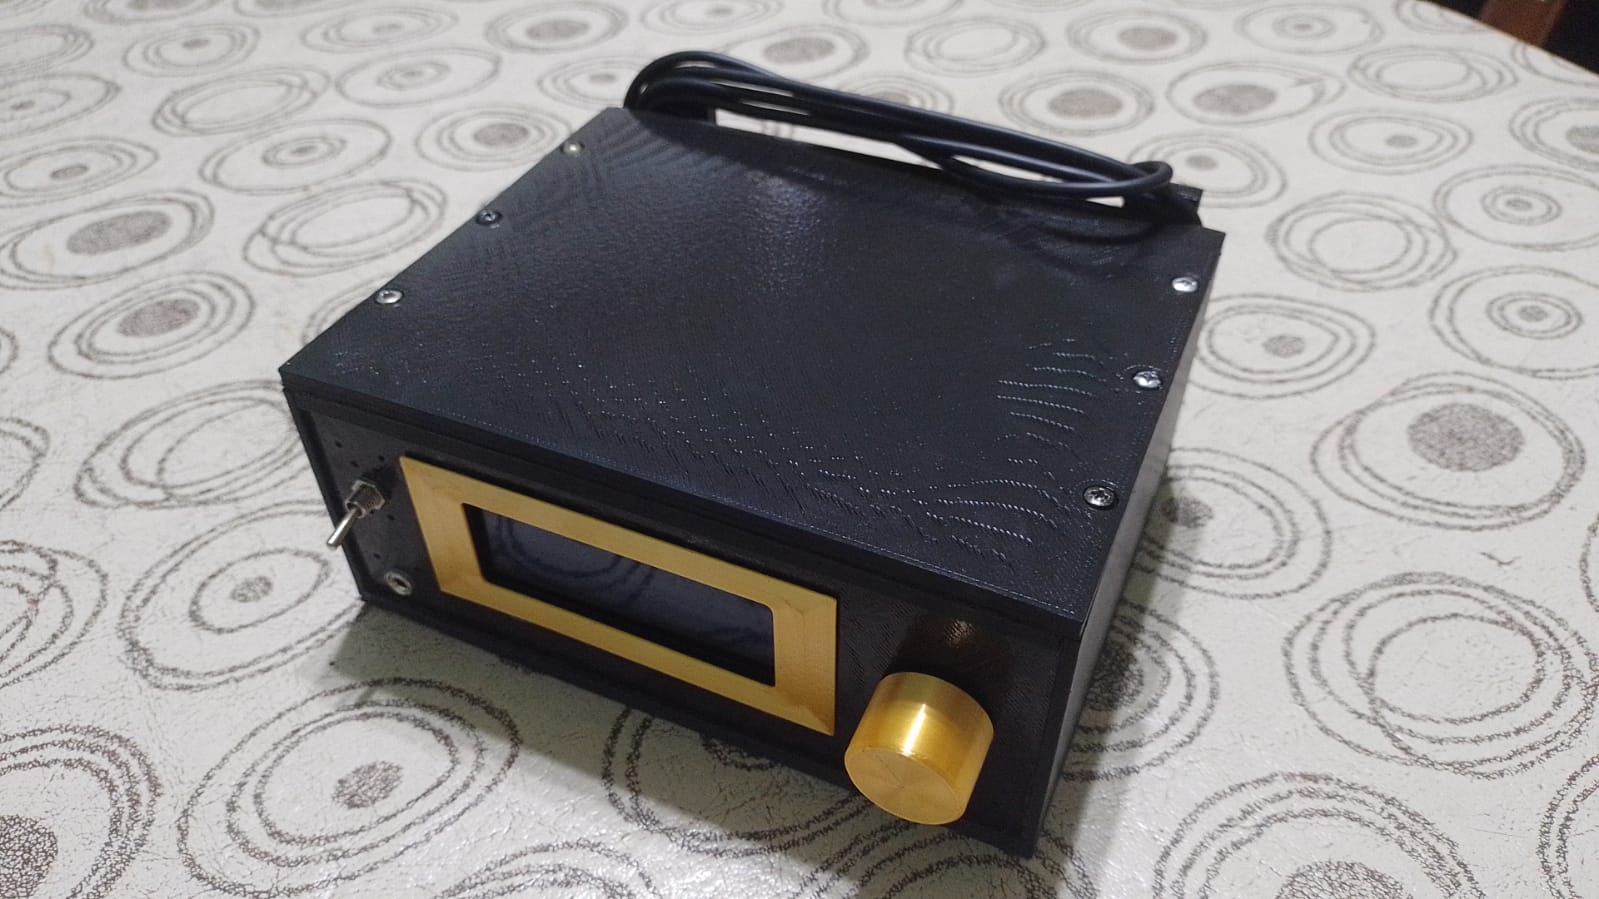
\includegraphics[width=0.7\linewidth]{producto final.png}
    \caption{Ensamble final}
    \label{fig:}
\end{figure}

% ============================================================
\section{Conclusiones}
Se ha desarrollado un sistema integrado que funciona en tiempo real y es controlable remotamente desde un sistema Linux. La interfaz gráfica proporciona una experiencia de usuario intuitiva y se lograron los objetivos propuestos por el alcance de manera satisfactoria. Dentro de las posibles mejoras al sistema estarían la inclusión de más bandas, mejorar la selectividad utilizando la version S3 del micro para aumentar la cantidad de taps del filtro y buscar un mejor aprovechamiento del rango dinámico del ADC y DAC para conseguir mejor rango que los $\pm$12 dB.


% ============================================================
\begin{thebibliography}{99}
\bibitem{intel386} Intel Corporation, \emph{80386 Programmer's Reference Manual}, Santa Clara, CA, 1990.
\bibitem{ldd3} J. Corbet, A. Rubini y G. Kroah-Hartman, \emph{Linux Device Drivers}, 3ra ed. Sebastopol, CA: O'Reilly Media, 2005.
\bibitem{pcm1808} Texas Instruments, \emph{PCM1808 Datasheet}, 2015.
\bibitem{pcm5102} Texas Instruments, \emph{PCM5102 Datasheet}, 2014.
\bibitem{smith_dsp} S. W. Smith, \emph{The Scientist and Engineer's Guide to Digital Signal Processing}, California Technical Publishing, 1997.
\bibitem{pcf8574} Texas Instruments, \emph{PCF8574T Datasheet}, 2015.
\bibitem{ky040} KY-040 Rotary Encoder Module Datasheet.
\bibitem{pl2303} Prolific, \emph{PL2303 Datasheet}.
\bibitem{rpi4} Raspberry Pi Ltd., \emph{Raspberry Pi 4 Model B Hardware Specifications and GPIO Pinout}, 2023.
\bibitem{egb} Cátedra de Técnicas Digitales III, \emph{Evaluación Globalizadora B: Sistemas Operativos de Propósito General}, UTN FRA, 2026.
\bibitem{task_not} freertos Documentation, \emph{FreeRTOS direct to task notifications}
\bibitem{gcc_aligned} Free Software Foundation, \emph{Variable Attributes -- Using the GNU Compiler Collection (GCC)}, 2008. [En línea]. Disponible en: \url{https://gcc.gnu.org/onlinedocs/gcc-4.3.2//gcc/Variable-Attributes.html}
\bibitem{esp_dsp_fir} Espressif Systems, \emph{ESP-DSP: Ejemplo de filtro FIR}. [En línea]. Disponible en: \url{https://github.com/espressif/esp-dsp/blob/3c12d059f96ec95ed00769fb32d41ca23e20cdf1/examples/fir/main/dsps_fir_main.c}
\bibitem{esp_dsp_speed} Espressif Systems, \emph{Issue oficial sobre velocidad de la librería ESP-DSP}, GitHub. [En línea]. Disponible en: \url{https://github.com/espressif/esp-dsp/issues/97}
\bibitem{smith_windowed_sinc} S. W. Smith, \emph{The Scientist and Engineer's Guide to Digital Signal Processing}, Cap. 16: Windowed-Sinc Filters. California Technical Publishing, 1997. [En línea]. Disponible en: \url{https://www.analog.com/media/en/technical-documentation/dsp-book/dsp_book_Ch16.pdf}
\end{thebibliography}

\end{document}